
\documentclass[palatino, bibnumbers]{apuntes}

\title{Geometría y Topología}
\author{Jose Antonio García del Saz}
\date{16/17 C2}
\usepackage{mathtools,tikz,lmodern, xparse}
\usetikzlibrary{%arrows, chains, matrix, 
	positioning, graphs,
	%shadows,
	shapes, shapes.callouts,
	%shapes.geometric,
	%shapes.misc
}
\usepackage{amsmath} %For align environement
\usepackage{color}% to define the next colors
\definecolor{bananayellow}{rgb}{1.0, 0.88, 0.21}
\definecolor{citrine}{rgb}{0.89, 0.82, 0.04}
\definecolor{darktangerine}{rgb}{1.0, 0.66, 0.07}

\newcommand{\Varrow}[3]{\begin{tikzpicture}[remember picture,overlay, ->, L/.style = {draw, #1}]
	\draw%[]
	(#2) edge[L] (#3); 
	\end{tikzpicture}       } 
% Paquetes adicionales
\usepackage{enumitem}
\usepackage{kpfonts}
\usepackage{tikztools}
\usepackage{fancysprefs}
\usepackage{tikz-3dplot}
\usepackage{physics}
\usepackage{xfrac}
\usepackage{wrapfig}
\usepackage{fastbuild}
\usepackage{soul}

%\usepackage{lipsum}
\usepackage{tikz-cd}
\usetikzlibrary{calc,patterns,angles,quotes}
\usetikzlibrary{arrows}
\usetikzlibrary{patterns}
\usetikzlibrary{intersections}
\usetikzlibrary{calc}
\usetikzlibrary{fadings}

\tikzset{
	snake/.style={
		rounded corners,
		to path={
			-- ([xshift=1em]\tikztostart.east)
			-- ([xshift=1em]\tikztostart.south east)
			-- ([xshift=-1em]\tikztotarget.north west)
			-- ([xshift=-1em]\tikztotarget.west)
			-- (\tikztotarget)
		}
	},
	snake up/.style={
		rounded corners,
		to path={
			-- ([xshift=-1em]\tikztostart.west)
			-- ([xshift=-1em]\tikztostart.north west)
			-- ([xshift=1em]\tikztotarget.south east)
			-- ([xshift=1em]\tikztotarget.east)
			-- (\tikztotarget)
		}
	}
}

\setlist{itemsep=1pt, topsep=5pt}
\bibliographystyle{alpha}
% --------------------

%\precompileTikz

\newcommand{\Id}{\mop{Id}}
\newcommand{\cln}{\colon\!}

\setcounter{tocdepth}{3}

\begin{document}
\pagestyle{plain}
\newcommand\tab[1][1cm]{\hspace*{#1}}
% http://tex.stackexchange.com/a/14243
\relpenalty=9999
\binoppenalty=9999
%\newcommand\restr[2]{\ensuremath{\left.#1\right|_{#2}}}
\begin{abstract}
Estos son los apuntes del curso de Geometría y Topología, del profesor Fernando Chamizo.
\end{abstract}

\maketitle

\tableofcontents
\newpage
% Contenido.

\chapter{Álgebra Tensorial}

\section{Tensores en  $ℝ^{n}$}
\subsection{Definiciones y ejemplos}
Estudiar los tensores en $ℝ^n$ es en realidad estudiar el Álgebra Lineal pero en varias variables. En primer curso (Álgebra I) estudiamos las aplicaciones, las cuales eran de la forma:
\begin{align*}
	\appl{π}{ℝ^{n}&}{ℝ^{m}} \\
	\overline{x} &\longmapsto[\overline{y}=A\cdot \overline{x}]
\end{align*}

\begin{defn}[Aplicación\IS lineal] Sea $f$ una aplicación entre dos espacios vectoriales $V$, $W$ sobre el mismo cuerpo $K$. Decimos que $f$ es una \textbf{aplicación lineal} si se cumplen las siguientes propiedades ($λ\in K$):
	\begin{enumerate}
		\item $f(λ\overline{x})=λ\cdot f(\overline{x})$ .
		\item $f(\overline{x_1}+\overline{x_2})=f(\overline{x_1})+f(\overline{x_2})$
	\end{enumerate}
\end{defn}

\begin{defn}[Aplicación\IS bilineal] Sea 
	\begin{align*}
	\appl{f}{ℝ^{n}×ℝ^{n}&}{ℝ} \\
	\overline{x},\overline{y} &\longmapsto{f(\overline{x},\overline{y})}
	\end{align*}
una aplicación, decimos que es \textbf{bilineal} si es una aplicación lineal en cada una de las dos variables, es decir:
\begin{enumerate}
	\item $f(λ\overline{x},\overline{y})=λ\cdot f(\overline{x},\overline{y})$; $f(\overline{x_1}+\overline{x_2},\overline{y})=f(\overline{x_1},\overline{y})+f(\overline{x_2},\overline{y})$
	\item $f(\overline{x},λ\overline{y})=λ\cdot f(\overline{x},\overline{y})$; $f(\overline{x},\overline{y_1}+\overline{y_2})=f(\overline{x},\overline{y_1})+f(\overline{x},\overline{y_2})$
\end{enumerate}
\end{defn}
\textbf{Observación:} todas las aplicaciones bilineales entre dos espacios se pueden escribir de la siguiente manera:
$$f(\overline{x},\overline{y})=\overline{x}^{T}A\overline{y}$$ con A una matriz n×n.
\newpage
\begin{defn}[Aplicación\IS multilineal] Decimos que una aplicación es \textbf{multilineal} si es lineal en cada una de sus variables. 
\end{defn}

\begin{defn}[Tensor\IS n veces covariante] Es cualquier aplicación multilineal
	$\appl{T}{\varprod_{i=1}^n V}{ℝ}$, siendo V un espacio vectorial de dimensión finita sobre $ℝ$ (que como sabemos de otros cursos son isomorfos a $ℝ^{n}$).
\end{defn}

\begin{example} Sea
	\begin{align*}
		\appl{T}{ℝ^{3}×ℝ^{3}&}{ℝ} \\
		T\left(\begin{pmatrix}x_1\\x_2\\x_3\end{pmatrix},\begin{pmatrix}y_1\\y_2\\y_3\end{pmatrix}\right) &\longmapsto{x_1\cdot y_3}
	\end{align*}
es obvio que T es multilineal, luego T es un tensor 2 veces covariante en $ℝ^{3}$.
\end{example}
\begin{example} Sea
	\begin{align*}
		\appl{T}{ℝ^{3}×ℝ^{3}&}{ℝ} \\
		T\left(\begin{pmatrix}x_1\\x_2\\x_3\end{pmatrix},\begin{pmatrix}y_1\\y_2\\y_3\end{pmatrix}\right) &\longmapsto{x_1\cdot x_3}
	\end{align*}
	se ve rápidamente que \underline{no} es una aplicación lineal respecto de la variable $\overline{x}$.
\end{example}
\begin{example} Sea
	\begin{align*}
		\appl{T}{ℝ^{3}×ℝ^{3}×ℝ^{3}&}{ℝ} \\
		T\left(\begin{pmatrix}x_1\\x_2\\x_3\end{pmatrix},\begin{pmatrix}y_1\\y_2\\y_3\end{pmatrix},\begin{pmatrix}z_1\\z_2\\z_3\end{pmatrix}\right) &\longmapsto{\begin{vmatrix}
			x_1 & y_1 &  z_1 \\ 
			x_2 & y_2 & z_2 \\ 
			x_3 & y_3 & z_3 \\ 
		\end{vmatrix}}
	\end{align*}
	la propiedad de linealidad del producto por un escalar es obvia por las propiedades de los determinantes. La propiedad de linealidad que conserva la adición se demuestra fácilmante desarrollando el determinante por adjuntos en la primera columna. Luego T es un tensor 3 veces covariante.
\end{example}
\newpage
En Álgebra Lineal estudiamos no sólo las aplicaciones $\appl{T}{ℝ^{n}}{ℝ}$ , sino también las de la forma $\appl{T}{ℝ^{n}}{ℝ^{m}}$. Ahora bien, estás últimas pueden convertirse al primer tipo mediante un elemento del \textbf{espacio dual}.

\begin{defn}[Espacio\IS dual] Sea V un espacio vectorial entonces se define el espacio dual y se denota con $V^{*}$ de la siguiente manera: \[ V^{*} = \{ \appl{f}{V}{ℝ} \tq \text{f es lineal} \}\]
\end{defn}

Con la definición anterior, un truco para pasar de unas aplicaciones a otras es que consideramos un elemento del espacio dual ($\phi\inℝ^{m}$) y uno del espacio vectorial original ($\overline{x}\inℝ^{n}$) y entonces tenemos una aplicación $$\hat{f}(\phi,\overline{x})=\phi(f(\overline{x}))\inℝ$$

De la misma manera, en lugar de considerar "tensores vectoriales" (esta expresión no es correcta, pero se da para ilustrar), los cuales serían aplicaciones multilineales $\appl{T}{\varprod_{1}^s V}{\varprod_{1}^r V}$, es más conveniente pensar en que el tensor va a depender también de los elementos del espacio dual. Luego vamos a considerar tensores de la forma $$\appl{T}{\underbrace{V^{*}×\cdots×V^{*}}_{\text{r veces}}×\underbrace{V×\cdots×V}_{\text{s veces}}}{ℝ}$$ que sean multilineales.

\begin{defn}[Tensor\IS r veces contravariante y s veces covariante] Es cualquier aplicación multilineal de la forma:
	$$\appl{T}{\underbrace{V^{*}×\cdots×V^{*}}_{\text{r veces}}×\underbrace{V×\cdots×V}_{\text{s veces}}}{ℝ}$$ siendo V un espacio vectorial de dimensión finita sobre $ℝ$ (isomorfo a $ℝ^{n}$) y $V^{*}$ su espacio dual. Diremos análogamente que T es un tensor de tipo (r,s).
\end{defn}

Como ya sabemos, si V es un espacio vectorial y tenemos una base de V (llamémosla $\base = \{ \overline{v_1},...,\overline{v_n} \}$), entonces existe una base natural de $V^{*}$
llamada \textbf{base dual} (denotada por $\base^{*}=\{\tilde{\phi}^{1},\cdots ,\tilde{\phi}^{n}\}$) y que está determinada por la propiedad: $$\tilde{\phi}^{i}(\overline{v_j})=\delta_j^{i} = \begin{cases} 0 & i ≠ j \\ 1 & i = j \end{cases}$$
\newpage
\begin{example} Daremos un ejemplo casi absurdo para ilustrar. Dar la base dual es muy fácil cuando tenemos una base ortonormal, por ejemplo la base canónica de $ℝ^{2}$:
$$\base = \{\overline{e_1},\overline{e_2}\}=\left\{\begin{pmatrix}1\\0\end{pmatrix},\begin{pmatrix}0\\1\end{pmatrix}\right\}$$En este caso obtenemos la base dual solamente girando los elementos de la base canónica, obteniendo: $$\base^{*} =\{\tilde{\phi^{1}},\tilde{\phi^{2}}\}=\left\{\begin{pmatrix}1&0\end{pmatrix},\begin{pmatrix}0&1\end{pmatrix}\right\}$$
\end{example}
\begin{example} Imaginemos que estamos en $ℝ^{2}$ pero en esta ocasión tenemos una cualquiera de sus bases $\base=\{\overline{v_1},\overline{v_2}\}$. Ahora consideramos la matriz $A=\begin{pmatrix}v_{11}&v_{21}\\v_{12}&v_{22}\\ \end{pmatrix}$, y entonces tenemos que $\begin{cases}\overline{v_1}=A\cdot \overline{e_1} \\\overline{v_2}=A\cdot \overline{e_2}\end{cases}$. Construímos entonces la base dual $\base^{*}=\{ \tilde{\phi^{1}},\tilde{\phi^{2}}\}$ de esta manera con la matriz de cambio de base: $\begin{cases} \tilde{\phi^{1}}(\overline{x})=\begin{pmatrix}0&1\end{pmatrix}\cdot A^{-1}\cdot \overline{x} \\\tilde{\phi^{2}}(\overline{x})=\begin{pmatrix}1&0\end{pmatrix}\cdot A^{-1}\cdot \overline{x}\end{cases}$
\end{example}
\begin{example} Si f es un \textit{endomorfismo}, digamos $\appl{f}{ℝ^{n}}{ℝ^{n}}$, se corresponde de manera unívoca con un tensor de tipo (1,1):
	\begin{align*}
	\appl{T}{(ℝ^{n})^{*}×ℝ^{n}&}{ℝ} \\
	T(\tilde{\phi},\overline{x}) &\longmapsto{\tilde{\phi}(f(\overline{x}))}
	\end{align*}
\end{example}
\begin{example} Cualquier vector de un espacio vectorial ($\overline{v}\in V$) se puede hacer corresponder con un tensor (1,0)  que se alimenta de elementos del dual y devuelve reales definido como:
	\begin{align*}
	\appl{T_{\overline{v}}}{V^{*}&}{ℝ} \\
	T_{\overline{v}}(\tilde{\phi}) &\longmapsto{\tilde{\phi}(\overline{v})}
	\end{align*}
\end{example}

Vamos a introducir notación para las definiciones y resultados venideros, y hay que hacerla nuestra ya que es el infierno de casi todos los estudiantes al abrir un libro de cálculo tensorial. De aquí en adelante (aunque se venga haciendo desde el inicio) se usarán \textbf{subíndices} para numerar vectores ($\overline{v_1},\overline{v_2},...,\overline{v_n}$) y \textbf{superíndices} para numerar elementos del espacio dual, aunque también sean vectores ($\tilde{\phi^{1}},\tilde{\phi^{2}},...,\tilde{\phi^{n}}$) .
\newpage
\begin{defn}[Componentes\IS de un tensor] Sea un tensor $T$ de tipo (r,s) y sean $\base=\{\overline{v_1},...,\overline{v_n}\}$, $\base^{*}=\{\tilde{\phi^{1}},...,\tilde{\phi^{n}}\}$ las bases de $V$ y $V^{*}$ respectivamente, se definen las componentes de $T$ en la base $\base$ como la siguiente colección de números:
	$$T_{j_1\space j_2\space \cdots \space j_s}^{i_1\space i_2\space \cdots \space i_r}=T(\tilde{\phi^{i_1}},\tilde{\phi^{i_2}},...,\tilde{\phi^{i_r}},\overline{v}_{j_1},\overline{v}_{j_2},...,\overline{v}_{j_s})$$
\end{defn}
\begin{example} Calcular las componentes del tensor:
	\begin{align*}
	\appl{D}{ℝ^{2}×ℝ^{2}&}{ℝ} \\
	D\left(\begin{pmatrix}x_1\\x_2\end{pmatrix},\begin{pmatrix}y_1\\y_2\end{pmatrix}\right) &\longmapsto{\begin{vmatrix}
		x_1 & y_1 \\ 
		x_2 & y_2 \\ 
		\end{vmatrix}}
	\end{align*}
	Lo primero que hacemos es coger una base (cogemos la canónica porque será lo más usual este curso). Como es un tensor (0,2), no habrá superíndices en las componentes, sólo subindices. Las componentes son: $$D_{j_1\space j_2}=\begin{cases}
		D_{1\space1}=D(\overline{e_1},\overline{e_1})=\begin{vmatrix}1&1 \\ 0&0 \\ \end{vmatrix}=0\\
		D_{1\space2}=D(\overline{e_1},\overline{e_2})=1\\
		D_{2\space1}=-1\\
		D_{2\space2}=0\\
	\end{cases}$$
\end{example}
\subsection{Convenio de Einstein}
Se usa para ahorrar en escritura cuando se habla del álgebra tensorial. En resumen consiste en que cuando se repite un índice arriba y abajo entonces hay que suponer que sumamos en él.
\begin{example} En primer curso, la combinación lineal se escribía como: $λ_1\cdot \overline{v_1}+\cdots +λ_n\cdot \overline{v_n}$. Si usamos el convenio esto se escribiría simplemente como $λ^{i}\cdot \overline{v}_i$
\end{example}
\begin{example} Sea una aplicación lineal $f(\overline{x})=A\cdot \overline{x}$, se corresponde unívocamente con un tensor (1,1):
	\begin{align*}
		\appl{T}{(ℝ^{n})^{*}×ℝ^{n}&}{ℝ} \\
		T(\tilde{\phi},\overline{v}) &\longmapsto{\tilde{\phi}(\overline{v})}
	\end{align*}
Las componentes (en la base canónica) son las $a_j^{i}$, donde $i$ son las filas y $j$ las columnas.
$$f(\overline{x})=a_j^{i}\cdot x^j;\overline{x}=x^j\cdot \overline{e_j}$$
Las componentes $T_j^{i}\equiv T(\tilde{\phi}^{i},\overline{e_j})=\begin{pmatrix}0&\cdots & 1 & \cdots &0\end{pmatrix}\cdot A\cdot \begin{pmatrix}
0 \\ \cdots \\ 1 \\ \cdots\\0\end{pmatrix}=a_j^{i}$
\end{example}
\newpage
\begin{example} Un tensor (1,3) muy importante es el llamado tensor de Riemann $\appl{T}{R=V^{*}×V×V×V}{ℝ}$. En relatividad $dim V = 4$ y tiene $4\cdot 4\cdot 4\cdot 4=256$ componentes y, para aplicarlo a un elemento del dual, digamos con componentes $(a_1,a_2,a_3,a_4)$, y a tres vectores, con coordenadas$(b_1,b_2,b_3,b_4), (c_1,c_2,c_3,c_4), (d_1,d_2,d_3,d_4)$, debemos escribir:
$$\sum_{i=1}^{4}\sum_{j=1}^{4}\sum_{k=1}^{4}\sum_{l=1}^{4}R_{j\space k\space l}^{i}a_i\space b^{j}\space c^{k}\space d^{l}$$
Esta expresión tiene demasiados sumatorios, si la reescribimos con el criterio de Einstein queda $R_{j\space k\space l}^{i}a_i\space b^{j}\space c^{k}\space d^{l}$\newline
\end{example}
\begin{defn}[Producto\IS tensorial] Sea T un tensor de tipo (r,s) y sea S otro tensor de tipo (u,v), de define su producto tensorial $T\otimes S$ como un nuevo tensor de tipo (r+u,s+v): $$T\otimes S(\tilde{\phi^{1}},\cdots ,\tilde{\phi^{r+u}})=T(\tilde{\phi^{1}},\cdots ,\tilde{\phi^{r}},\overline{v}_1,\cdots,\overline{v}_s)\cdot S(\tilde{\phi^{r+1}},\cdots ,\tilde{\phi^{r+u}},\overline{v}_{s+1},\cdots,\overline{v}_{s+v})$$
\end{defn}
\begin{example}Tomaremos estos dos tensores de tipo (0,1) en $ℝ^{2}$: $$T(\overline{x})=2\cdot x^{1}+x^{2}; S(\overline{x})=5\cdot x^{1}$$ y hallaremos ahora las componentes de $T\otimes S$, que será por definición un nuevo tensor de tipo (0,2), de la forma $\appl{T\otimes S}{ℝ^{2}×ℝ^{2}}{ℝ}$, y le llamaremos P a partir de ahora. Entonces tenemos que: $$\begin{cases}
	P_{1\space1}=P(\overline{e}_1,\overline{e}_1)=10\\
	P_{1\space2}=0\\
	P_{2\space1}=P(\overline{e}_2,\overline{e}_1)=5\\
	P_{2\space2}=0\\
	\end{cases}$$
	
\end{example}
\begin{example}En física e ingeniería se consideran muchos tensores importantes. Por ejemplo, el \textbf{tensor de inercia} es un tensor de tipo (0,2) que mide (entre otras cosas) lo difícil que es girar un sólido rígido respecto a un eje dado (en términos físicos es difícil si necesito un gran \textbf{trabajo} para girarlo).\\
	$$
	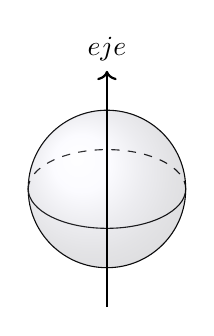
\begin{tikzpicture}
	\draw (-1,0) arc (180:360:1cm and 0.5cm);
	\draw[dashed] (-1,0) arc (180:0:1cm and 0.5cm);
	\draw (0,0) circle (1cm);
	\shade[ball color=blue!10!white,opacity=0.20] (0,0) circle (1cm);
	\draw[thick,->] (0,-1.5,0) -- (0,1.5,0) node[above]{$eje$};
	\end{tikzpicture}
\tab
	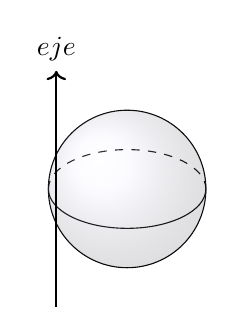
\begin{tikzpicture}
	\draw (-1,0) arc (180:360:1cm and 0.5cm);
	\draw[dashed] (-1,0) arc (180:0:1cm and 0.5cm);
	
	\draw (0,0) circle (1cm);
	\shade[ball color=blue!10!white,opacity=0.20] (0,0) circle (1cm);
	\draw[thick,->] (-0.9,-1.5,0) -- (-0.9,1.5,0) node[above]{$eje$};
	\end{tikzpicture}
	$$
Por ejemplo, en la figura, suponiendo que es una esfera que pesa toneladas, la intuición nos dice sin hacer cálculos que costará menos rotar la esfera respecto al primer eje que rotarla respecto al segundo (y estamos en lo cierto).
\end{example}
\begin{example}Los tensores también aparecen en el \textbf{entrelazamiento cuántico}, dentro del campo de la mecánica cuántica.
Una partícula se corresponde con un vector, que como sabemos se corresponde con un tensor (1,0). Pues si tenemos dos partículas $\overline{v}$ y $\overline{w}$, entonces el sistema formado por ambas partículas es  $\overline{v}\otimes\overline{w}$.
\end{example}
\section{Repaso (intuitivo) de Geometría Diferencial}
Empezaremos con el objeto matemático al que llamamos \textbf{variedad}. Como idea, una variedad es un objeto geométrico que se puede parametrizar por abiertos de $ℝ^{n}$, pero el gran salto con respecto de la geometría de la asignatura de GCS, es que la variedad no está inmersa en $ℝ^{n}$, sino que está ahí (como el universo), sin preocuparnos lo que sea que la rodea.\newline
\indent La idea de variedad diferenciable n-dimensional es, por tanto, la de un objeto geométrico compuesto por parches que son similares a abiertos de $ℝ^{n}$. Partimos de un espacio topológico M al que exigimos que tenga la propiedad de Hausdorff y una base numerable (segundo axioma de numerabilidad). La primera propiedad es natural si queremos poder tratar separadamente los puntos, y las segunda va también en este sentido, porque permite asegurar la existencia de particiones de la unidad, que son totalmente necesarias para hacer el an análisis local típico de la geometría diferencial.
Una carta nos dice la manera de allanar un parche de M en $ℝ^{n}$ (es la inversa de la parametrización en ese abierto de $ℝ^{n}$).
$$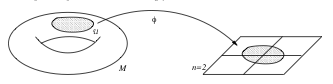
\includegraphics[width=\linewidth]{img/GT17_Variedad_carta}$$
El número de parámetros que la parametrización requiere es llamado en geometría \textbf{dimensión} de la variedad (mientras en mecánica lo llamaríamos \textbf{grados de libertad}). Si llamamos $\phi$ a la inversa de la parametrización (la carta), entonces tendremos (mirar figura superior) algo como $\phi(x^{1},\cdots,x^{n})$, que nos lleva a $ℝ^{n}$ y donde $x^{i}$ son lo que llamamos \textbf{funciones coordenadas}. Vamos a formalizarlo rápidamente para no empezar a divagar.

\begin{defn}[Carta\IS n-dimensional] Una carta n-dimensional de M es un par $(\mathcal{U},\phi)$ donde $\mathcal{U}$ es un abierto
de M y $\phi$ es una función $\appl{\phi}{\mathcal{U}}{ℝ^{n}}$ que es homeomorfismo sobre su imagen.
\end{defn}

Como un punto puede estar tapado por varios parches, diferentes abiertos de cartas, debemos asegurarnos de que el análisis no se estropea bajando por una $\phi$ o por otra. Una de las cosas que se suelen pedir en Geometría Diferencial es que si existe otra parametrización $\psi$, entonces tanto $\psi\circ\phi$ como $\phi\circ\psi$ han de ser de clase $C^{\infty}$ (En el abierto intersección de $ℝ^{n}$), y en ese caso se dice que las cartas son \textbf{compatibles} 

\begin{defn}[Derivada parcial i-ésima en una variedad] Se dice que una función $\appl{f}{M}{ℝ}$ es $C^{\infty}$ si para cada carta $(\mathcal{U},\phi)$ la función $\appl{f\circ \phi^{-1}}{\phi(\mathcal{U})}{ℝ}$ lo es, y se define para cada $p \in \mathcal{U}$ la derivada parcial i-ésima en la variedad como $$\restr{\pdv{f}{x^{i}}}{p}=D_i(f\circ \phi^{-1})(\phi(p))$$ donde $D_i$ denota la derivada parcial usual respecto de la variable i-ésima.
\end{defn}

No daremos la definición rigurosa, pero sí diremos que a las funciones $C^{\infty}$ entre dos variedades $M$ y $N$ que tienen inversa $C^{\infty}$ se llaman \textbf{difeomorfismos}
\newpage
Un problema técnicamente más complejo es la definición del \textbf{espacio tangente}, que en el caso de subvariedades de $ℝ^{n}$ es muy fácil. No es una mera adaptación porque allí los vectores tangentes eran “pelos” orientados que se salían de la subvariedad, mientras que ahora concebimos las variedades como una entidad única, sin referencia a un posible “exterior”. Hay varias maneras de superar este obstáculo. Aquí mencionaremos las definiciones matemáticas que corresponden a ver los vectores tangentes como velocidades de curvas y como derivadas direccionales. La segunda es más abstracta, se hace introduciendo implícitamente el concepto de derivación.

\begin{defn}[Espacio\IS tangente de una variedad] Se llama espacio tangente de una variedad M en un punto p al conjunto cociente $T_p(M)=K_p(M) /\sim$ donde $K_p(M)=\{ $Funciones $\appl{c}{(-\epsilon,\epsilon)}{M}$ con $c(0)=p \}$ y $\sim$ identifica las funciones curvas tales que $(\phi\circ c_1)'(0)=(\phi\circ c_2)'(0)$ con $(\mathcal{U},\phi)$ una carta. Se llama \textbf{vector tangente} de M en p a cualquiera de sus elementos.
\end{defn}

\begin{defn}[Vector\IS tangente en una variedad] Se llama vector tangente de $M$ en $p$ a cualquier operador $ℝ$-lineal $\appl{v}{E_p(M)}{ℝ}$ que satisface $v(fg)=v(f)g(p)+f(p)v(g)$ para todo $f,g \in E_p(M)$, donde $E_p(M)$ es el anillo de funciones $M\longmapsto ℝ$ definidas en un entorno suficientemente pequeño de p. Se llama espacio tangente de $M$ en un punto $p$ al conjunto formado por todos los vectores tangentes.
\end{defn}

A partir de las curvas que corresponden a los ejes coordenados (una vez que bajamos a $ℝ^{n}$ por la carta) se obtienen unos vectores tangentes que denotaremos con el extraño nombre $\restr{\pdv{}{x^{i}}}{p}$. Para ser rigurosos, si $\{\overline{e}_1,\overline{e}_2,\cdots,\overline{e}_n\}$ es la base canónica, fijada una carta $(\mathcal{U},\phi=(x^1,\cdots,x^n))$ con la primera definición se tiene $$\restr{\pdv{}{x^{i}}}{p}=[c_i]\tab con \tab c_i(t)=\phi^{-1}(\phi(p)+t\overline{e}_i),\tab i=1,2,...,n $$

Denominar a estos vectores con el mismo símbolo que el de las derivadas parciales no es casual, pues con la segunda definición no son más que las derivadas parciales i-ésimas en la varidad, es decir 
\begin{equation}
\appl{\restr{\pdv{}{x^{i}}}{p}}{f}{\restr{\pdv{f}{x^{k}}}{p}}
\end{equation}
Por razones obvias se les suele denotar con la notación abreviada $\restr{\partial_i}{p}$, o incluso $\partial_i$ si el punto no se indica.
\begin{prop} El espacio tangente $T_p(M)$ tiene una estructura natural de espacio vectorial cuya dimensión es la de la variedad diferenciable M.
\end{prop}
\begin{prop} Para cada punto p de una variedad diferenciable n-dimensional $M$, el conjunto $\{\restr{\partial_1}{p},\restr{\partial_2}{p},\cdots,\restr{\partial_n}{p}\}$ es una base de $T_p(M)$.
\end{prop}
Hasta aquí , si aún no nos hemos quitado la vida con la notación, podemos proceder.
\newpage
Con $\appl{f}{M}{N}$ podemos pasar curvas en curvas lo cual induce una aplicación $T_p(M)\longmapsto T_{f(p)}(N)$. Aunque ésta es la idea intuitiva, es más sintético proceder tomando en cuenta la segunda definición de espacio tangente.

\begin{defn}[Aplicación\IS tangente] Sea $\appl{f}{M}{N}$. Se llama aplicación tangente de f en p y se denota con $\restr{\dv{f}}{p}$, a la aplicación lineal $T_p(M)\longmapsto T_{f(p)}(N)$ que aplica un elemento de $T_p(M)$ (considerado con la segunda definición), digamos $v(\cdot)$ en $v(\cdot\circ f)$
\end{defn}
\begin{prop} Sea $\appl{f}{M}{N}$ y sean $(\mathcal{U}(p),\phi)$ y $(\mathcal{V}(f(p)),\psi)$ cartas de M y N respectivamente en los puntos indicados. La matriz de la aplicación tangente $\restr{df}{p}$ en las bases $\{\restr{\pdv{}{x^1}}{p},\cdots,\restr{\pdv{}{x^m}}{p}\}$ y $\{\restr{\pdv{}{y^1}}{f(p)},\cdots,\restr{\pdv{}{y^n}}{f(p)}\}$ correspondientes a estas cartas es la matriz jacobiana de $\psi\circ f\circ\phi^{-1}$ en $\phi(p)$.
\end{prop}

Dada una carta $(\mathcal{U},\phi=(x^1,\cdots,x^n))$ de M tiene sentido considerar las aplicaciones tangentes de las funciones coordenadas $\restr{dx^{i}}{p}$ como funciones de $M$ en $ℝ$ con la estructura de variedad obvia. Usando las definiciones de vector tangente se puede probar que $$\restr{dx^{i}}{p}(\restr{\pdv{}{x^j}}{p})=\delta_j^i$$ o dicho de otra forma $$\{\restr{dx^1}{p},\restr{dx^2}{p},\cdots,\restr{dx^n}{p}\}\tab \text{es la base dual de} \tab\{\restr{\pdv{}{x^1}}{p},\restr{\pdv{}{x^2}}{p},\cdots,\restr{\pdv{}{x^n}}{p}\}$$

\begin{defn}[Espacio\IS cotangente] Dada una carta $(\mathcal{U},\phi=(x^1,\cdots,x^n))$ de $M$, al espacio vectorial sobre $ℝ$ generado por $\{\restr{dx^1}{p},\restr{dx^2}{p},\cdots,\restr{dx^n}{p}\}$ se denomina espacio cotangente de M en p y se denota con $T_p^{*}(M)$, por ser el dual de $T_p(M)$.
\end{defn}

\begin{defn}[Uno forma] Los elementos de $T_p^{*}(M)$ se llaman uno formas (o covectores).
\end{defn}

Como cabía esperar, en lo sucesivo descargaremos la notación para las aplicaciones tangentes y las bases introducidas de $T_p(M)$ y $T_p^{*}(M)$ omitiendo el punto cuando no sea relevante. Por ejemplo, escribiremos $dx^1$ en lugar de $\restr{dx^1}{p}$.

Una vez más insistimos en que todos los espacios vectoriales sobre $ℝ$ son lo mismo, y una vez fijadas las bases las operaciones se realizan coordenada a coordenada como nos enseñaron en primero cuando casi todo era con vectores de $ℝ^{n}$. Los elementos del dual no albergan nada nuevo y siguen funcionando como se indicó en la sección anterior (y en el curso de primero) por mucho que pongamos $d$ y $\partial$ por todos los lados. En un ejemplo: \\ $$(2dx^1+3dx^2)(2\pdv{}{x^1}-\pdv{}{x^2})=1 \tab\text{porque}\tab \begin{pmatrix}2&3\end{pmatrix}\begin{pmatrix}2\\-1\end{pmatrix}=1$$
\newpage
\section{Tensores en el espacio tangente}
Ya hemos visto tensores en $ℝ^{n}$, veamos que pasa cuando consideramos los tensores en las variedades en general. Podemos considerar tensores cuyo espacio vectorial subyacente sea el espacio tangente de la variedad en cada punto, y cuyo dual es el cotangente: $$V=T_p(M)\tab V^*=(T_p(M))^*$$
Será conveniente permitir variar el punto y tener entonces un \textbf{campo de tensores} (un tensor definido en cada punto de la variedad) y queremos que sea diferenciable (en algún sentido).\\ 
Para hacer la teoría más sintética, es conveniente introducir el \textbf{fibrado}, tanto tangente como cotangente: $$TM=\bigcup\limits_{p\in M} T_p(M)\tab T^*M=\bigcup\limits_{p\in M} (T_p(M))^* $$ con cierta estructura de variedad. En física a esto se le llama \textbf{espacio de fases} (partículas elementales).

\begin{defn}[Tensor\IS en una variedad] Sea $M$ una variedad. Un tensor (en rigor, campo tensorial) $C^{\infty}$ de tipo $(r,s)$ en $M$ es una aplicación que a cada punto $p$ le asigna un tensor de tipo $(r,s)$ con $V=T_p(M)$ y $V^*=(T_p(M))^*$ y tal que en cada carta las componentes sean funciones $C^{\infty}$.
\end{defn}

\begin{defn}[Métrica] Una métrica en una variedad es un tensor de tipo (0,2) en dicha variedad tal que si en una carta $(g_{i\space j})$ es la matriz de componentes, entonces esta matriz es simétrica y no singular.
\end{defn}

\begin{example}En $ℝ^{2}$ con la carta identidad tenemos $G=dx\otimes dx+dy\otimes dy$. Tomemos $\overline{v}=a^i\pdv{}{x^i}$ y $\overline{w}=b^i\pdv{}{x^i}$, ambos en $ℝ^{2}$, y entonces con la métrica G: $$G(\overline{v},\overline{w})=dx(\overline{v})\cdot dx(\overline{w})+dy(\overline{v})\cdot dy(\overline{w})=a^1+b^1\cdot a^2+b^2$$ que es el producto escalar usual.
\end{example}
\begin{example}\textbf{(Métrica de Poincaré)}\indent En $ℝ×ℝ^+$ se define la métrica:\space$G=y^{-2}(dx\otimes dx+dy\otimes dy)$. Sea $\overline{v}=3\restr{\pdv{}{x}}{p}+\restr{4\pdv{}{y}}{p}$; para $p=(0,1)$; entonces $G(\overline{v},\overline{v})=3^2+4^2=25$. Y si $\overline{w}=3\restr{\pdv{}{x}}{q}+\restr{4\pdv{}{y}}{q}$; para $q=(0,5)$; entonces $G(\overline{w},\overline{w})=1$.
\end{example}
\begin{example}\textbf{(Métrica alrededor de un agujero negro)}\indent Se define como $$G=-\left(1-\frac{r_0}{r}\right)dt\otimes dt+\left(1-\frac{r_0}{r}\right)^{-1}dr\otimes dr$$ donde r es la distancia al centro, t es el tiempo y $r_0$ una constante.
\end{example}
\newpage
\begin{example}\textbf{(Componentes de la métrica usual en $ℝ^2$ )}\indent Tenemos la métrica usual del producto escalar con componentes: $$\begin{cases}
	g_{1\space1}=1 \tab g_{1\space2}=0\\
	g_{2\space1}=0 \tab g_{2\space2}=1\\
	\end{cases}$$
	En general, una métrica es de la forma $G=g_{i\space j}dx^i\otimes dx^j$. En la matriz de componentes de la métrica usual nos encontramos con la identidad (simétrica y no singular).
\end{example}

\begin{example}\textbf{(Componentes de la métrica de Poincaré )}\indent Se tienen las componentes:$$G=(g_{i\space j})=\begin{pmatrix}y^{-2}&0\\0&y^{-2}\\ \end{pmatrix}$$ Lo mas importante de los tensores en variedades es saber como se comportan sus componentes por cambios de carta.
\end{example}

Si tenemos un tensor T en una variedad M para cierta carta, el tensor no depende de la carta pero las componentes si: $$\tilde{T}^{i_1,\cdots,i_r}_{j1,\cdots,j_s}=\pdv{y^{i_1}}{x^{k_1}}\cdots\pdv{y^{i_r}}{x^{k_r}}\pdv{x^{l_1}}{y}\cdots\pdv{x^{l_s}}{y^{j_s}}\cdot T^{k_1,\cdots,k_r}_{l_1,\cdots,l_s},\tab\text{para }\psi=(y^1,\cdots,y^n)$$
Esto se deduce por la regla de la cadena de la sigiente manera: $$\pdv{y^j}=\pdv{x^i}{y^j}\pdv{x^i};\tab dy^j=\pdv{y_j}{x^i}dx^i;$$
Por definición tendriamos que $\tilde{T}^{i_1\cdots i_r}_{j_1,\cdots,j_s}=T(dy^{i_1},\cdots,dy^{i_r},\pdv{y^{j_1}},\cdots,\pdv{y^{j_s}})$.
Si recordamos la definición de métrica como tensor $(0,2)$ en una variedad cuya matriz de componentes es simétrica y no singular nos preguntamos si podemos pasar los tensores de una variedad $M$ a tensores en una variedad $N$ por medio de una aplicación. Y la respuesta es que no es tan trivial como parece. 

\begin{defn}[Pull-back] Sea un tensor $T$ de tipo $(0,s)$ en la variedad N, se llama pull-back (o en español menos popularmente imagen recíproca) al tensor de tipo $(0,s)$ en $M$ definido por la siguiente expresión: $$f^*T(\overline{v}_1,\cdots,\overline{v}_s)=T(df(\overline{v}_1),\cdots,df(\overline{v}_s))$$
\end{defn}

El pull-back será muy interesante cuando estudiemos las formas diferenciables. Para los tensores $(r,s)$ no está bien definida por no saber como tratar con los elementos del dual, y para los de tipo $(r,0)$ hay otra cosa definida que se llama push-forward.
\newpage
\begin{defn}[Métrica\IS inducida] Sea $i$ una inclusión, y sea $T=G$ una métrica, se dice que $i^*G$ es la métrica inducida.
\end{defn}

\begin{example} Sean 
	\begin{tikzcd}
	\mathbb{S}^1 \arrow[r] \arrow[d, "\phi=ang."] & ℝ^2 \arrow[d, "\psi=id"] \\
		\theta & (x,y)
	\end{tikzcd} 
y la métrica usual en $ℝ^2$: $G=dx\otimes dx+dy\otimes dy$\\
En lugar de seguir la fórmula de la definición de pull-back recordamos que la aplicación tangente usa las derivadas parciales (el jacobiano). Tenemos pues:\\
$$\begin{cases}
x=cos (\theta)\\
y=sen(\theta)\\
\end{cases}\mapsto
\begin{cases}
dx=-sen (\theta)\\
dy=cos(\theta)\\
\end{cases}$$
Cabe decir que la llave izquierda no es un cambio de carta, es la inclusión $\psi\circ i\circ \phi^{-1}$. Concluyendo, tenemos la métrica inducida por la usual en $\mathbb{S}^1$:
$$i^*G=(-sen(\theta))^2d\theta\otimes d\theta + (cos^2(\theta))d\theta\otimes d\theta=d\theta\otimes d\theta$$ 
\end{example}
\begin{example}\textbf{(Típico de GCS: Superficie inmersa en $ℝ^3$ )}\\ 
	\begin{wrapfigure}{r}{0.5\textwidth}
		\begin{center}
			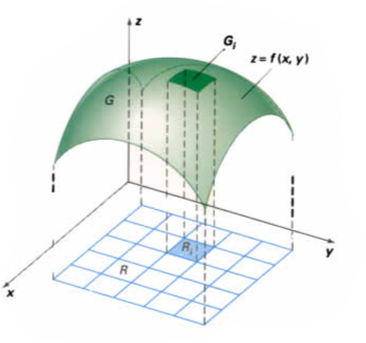
\includegraphics[width=0.40\textwidth]{img/GT17_parametric_surface}
		\end{center}
		\caption{Superficie inmersa en $ℝ^3$ }
	\end{wrapfigure}
Llamamos (u,v) a los parámetros de la superficie, que en la foto aparecen como $(x,y)$:\\
$\begin{cases}
x=f^1(u,v)\\
y=f^2(u,v)\\
z=f^3(u,v) \\
\end{cases}$
$\begin{cases}
dx=\pdv{f^1}{u}du+\pdv{f^1}{v}dv\\
dy=\pdv{f^2}{u}du+\pdv{f^2}{v}dv\\
dz=\pdv{f^3}{u}du+\pdv{f^3}{v}dv \\
\end{cases}$
\\La métrica inducida por la usual (que para confundirnos aún más recibe también el nombre de usual) es la suguiente:\\ \\
$i^*(dx\otimes dx+dy\otimes dy+dz\otimes dz)=$$$(\pdv{f^1}{u}du+\pdv{f^1}{v}dv)\otimes(\pdv{f^1}{u}du+\pdv{f^1}{v}dv)\cdots=$$\\$\left(\norm{\pdv{f}{u}}\right)^2du\otimes du+\cdots$
\end{example}

Como se ha visto en los ejemplos, en la práctica es mucho más cómodo aplicar las siguientes fórmulas que la ley general de transformación de tensores:
$\begin{cases}
\pdv{y^j}=\pdv{x^i}{y^j}\pdv{x^i}\\
dy^j=\pdv{y_j}{x^i}dx^i\\
\end{cases}$
\newpage
\begin{example}Vamos a cambiar la métrica usual de $ℝ^2$ a polares (y como venimos haciendo, pasamos de la fórmula del pull-back). Tenemos la métrica $G=dx\otimes dx+dy\otimes dy$ y el cambio de carta $\begin{cases}
	x=r\cdot cos (\theta)\\
	y=r\cdot sen(\theta)\\
	\end{cases}\mapsto
	\begin{cases}
	dx=cos(\theta)dr-sen(\theta)d\theta\\
	dy=sen(\theta)dr+cos(\theta)d\theta\\
	\end{cases}$\\
	Si sustituímos en la métrica usual tenemos: $$cos^2(\theta)dr\otimes dr+r^2sen^2(\theta)d\theta\otimes d\theta+sen^2(\theta)dr\otimes dr+r^2cos^2(\theta)d\theta\otimes d\theta=dr\otimes dr+r^2d\theta\otimes d\theta$$
\end{example}
\chapter{Geometría Riemanniana}
\section{Cálculo de variaciones y mecánica}
El cálculo de variaciones se dedica a hallar máximos y mínimos de \textbf{funcionales} (entendiendo esta palabra como aplicación que va de un espacio de funciones a $ℝ$). Lo más común es el ejercicio en el que hay que minimizar una integral (como hallar el "tobogán" más rapido entre dos puntos dados), aunque hay otros como intentar hallar el área máxima que podemos encerrar con una cuerda de longitud 1 (Demostrar que la solución es una circunferencia no es trivial sin el cálculo de variaciones). 
\begin{obs}Durante este capítulo, se usara la notación $\dot{f}\equiv\dv{f}{t}$
\end{obs}
\begin{example}\textbf{(Problema de la Braquistócrona I)}\\
\begin{wrapfigure}{r}{0.5\textwidth}
		\begin{center}
			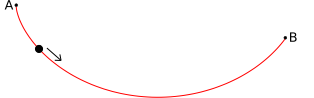
\includegraphics[width=0.5\textwidth]{img/GT17_Brachistochrone}
		\end{center}
		\caption{Curva Braquistócrona}
\end{wrapfigure}
Una curva braquistócrona, o curva del descenso más rápido, es la curva entre dos puntos que es recorrida en menor tiempo (el "tobogán" del que hablábamos antes), por un cuerpo que comienza en el punto inicial con velocidad cero, y que debe desplazarse a lo largo de la curva hasta llegar al segundo punto, bajo acción de una fuerza de gravedad constante y suponiendo que no existe fricción.\\ \\ \indent Supongamos que dicha curva es la gráfica de una función $y=f(x)$ en $ℝ^2$ y entonces el problema consiste en minimizar el tiempo que se tarda en ir de $A$ a $B$. Dicho tiempo (llamémosle $T$) se corresponde con la integral: $$\int_{0}^{1}\sqrt{\frac{1+(\dot{f}(x))^2}{2g\cdot f(x)}}dx;\tab\text{donde g es la constante gravitacional.}$$ 
\end{example}

A continuación se enuncia la proposición básica del cálculo de variaciones.
\newpage
\begin{prop} Dados $a,b\inℝ$; $\overline{c},\overline{d}\in ℝ^n$ y un conjunto de funciones $$\mathcal{C}=\{F=(q^1,\cdots,q^n)\space:\space F(a)=\overline{c},\space F(b)=\overline{d}\}$$ Supongamos además que tenemos la integral $$\int_{a}^{b}L dt;\tab\text{con }L=L(t,F(t),\dot{F}(t))$$ y que esta alcanza un máximo o un mínimo en $\mathcal{C}$, entonces dicha F es solución de la versión discreta (la que se usa en mecánica clásica) de \textbf{Euler-Lagrange}:
\begin{equation}
\label{eq:Euler-Lagrange}
\dv{t}\left(\pdv{L}{\dot{q^i}}\right)=\pdv{L}{q^i};\tab i=1,\cdots,n
\end{equation}
\end{prop}

\begin{proof}Sea $f(\epsilon)=\int_{a}^{b}L(t,F_0(t)+\epsilon\alpha t,\dot{F}_0(t)+\epsilon\dot{\alpha}(t))dt$; siendo $F_0$ la función para la que se alcanza el extremo y siendo $\appl{\alpha}{[a,b]}{ℝ^n}$ arbitraria con $\alpha(a)=\alpha(b)=0$; $\appl{f}{I}{ℝ}$ alcanza un extremo en $\epsilon=0$, por tanto:
	$$\dot{f}(0)=0\longrightarrow0=\int_{a}^{b}\left(\pdv{L}{q^i}\alpha^i+\pdv{L}{\dot{q}^i} \dot{\alpha}^i \right)dt=\int_{a}^{b}\left(\pdv{L}{q^i}-\dv{t}\left(\pdv{L}{\dot{q}^i}\right)\dot{\alpha}^i \right)dt$$
	que implica las ecuaciones de Euler-Lagange.
\end{proof}

\begin{example}$$I=\int_{1}^{2}(1+t^2(\dot{q}(t))^2)dt;\tab q(1)=2, q(2)=3$$
	Hay que encontrar la $q=q(t)$ que minimiza I. ¿Cuál es? Pues atendiendo a la proposición llamamos $L$ al integrando y tenemos siguiendo la fórmula: $$L=1+t^2\dot{q}^2\longrightarrow\begin{cases}
	\pdv{L}{\dot{q}}=2t^2\dot{q};\\
	\pdv{L}{q}=0;
	\end{cases}\longrightarrow\dv{t}(2t^2\dot{q})=0;$$
	Luego nos queda la EDO $4t\dot{q}+2t^2\ddot{q}=0$ y solo hay que resolverla. Tenemos que $t^2\dot{q}=cte\rightarrow \dot{q}(t)=\frac{cte}{t^2}$. Luego ya podemos integrar para hallar la función deseada: $$q(t)=K_1+\frac{K_2}{t}\xrightarrow{q(1)=2, q(2)=3}q(t)=4-\frac{2}{t}$$
Con esta q tenemos que I=3. Por ejemplo, si hubieramos cogido $q(t)=t+1$, entonces tendríamos $I=\frac{10}{3}\textgreater3$.\\
\end{example}
Volvamos ahora al ejemplo de la Braquistócrona.
\begin{example}\textbf{(Problema de la Braquistócrona II)}\\
Teníamos que:
$$\int_{0}^{1}\sqrt{\frac{1+(\dot{f}(x))^2}{2g\cdot f(x)}}dx;\tab f(0)=1,f(1)=0$$ 
\newpage
Luego tenemos que nuestro integrando, al que venimos llamando $L$, es:
$$L=\sqrt{\frac{1+(\dot{q}(x))^2}{2g\cdot q(x)}}\longrightarrow\begin{cases}\pdv{L}{\dot{q}}=\frac{1}{\sqrt{2gq}}\frac{\dot{q}}{\sqrt{1+\dot{q}^2}}\\
\pdv{L}{q}=\sqrt{\frac{1+(\dot{q}(x))^2}{2g}}\cdot\frac{-1}{2}\cdot q^{\frac{-3}{2}}
\end{cases}$$
Y si ahora usamos las ecuaciones de Euler-Lagrange nos sale una EDO bastante complicada. Para ayudar damos una proposición nueva
\end{example}
\begin{prop}\textbf{(Ley de conservación de la energía)} Supongamos que $L$ no depende explícitamente de $t$. Por tanto, $L(t,q,\dot{q})=L(q,\dot{q})$ y entonces a lo largo de cualquier solución de las ecuaciones de Euler-Lagrange se cumple que:
\begin{equation}
\label{eq:ConservacionEnergia}
\dot{q}^i\pdv{L}{\dot{q}^i}-L=cte
\end{equation}
\end{prop}
\begin{proof}
	$\dv{t}\left(\dot{q}^i\pdv{L}{\dot{q}^i}-L\right)=\ddot{q}^i\pdv{L}{\dot{q}^i}$Por terminar...
\end{proof}
HASTA AQUÍ EL PRIMER EXAMEN PARCIAL\\
¿Por qué pueden interesarnos estos resultados del cálculo de variaciones en geometría de variedades? Imaginemos que tenemos el problema anterior, en el que intentabamos minimizar $\int_{1}^{2}(1+t^2(\dot{q}(t))^2)dt$, donde $L=1+t^2\dot{q}^2$ y el mínimo era 3.
Ahora, si cambiamos de nombre la función incógnita $q$, el mínimo debería seguir siendo el mismo. Entonces yo podría considerar (por ejemplo, yo,porque quiero) llamar a la $q=h^2$  (suponiendo que esto funciona bien: como $q$ es positiva se puede escribir como un cuadrado...) y el mínimo debería ser el mismo y alcanzarse para la misma función. El nuevo $\tilde{L}=1+t^2(2h\dot{h})^2$ y el mínimo debe salir el mismo salvo el cambio de nombre. Si antes $q(t)=4-\frac{2}{t}$ ahora $h(t)=\sqrt{4-\frac{2}{t}}$. Esto es sorprendente porque si cambio las coordenadas en las ecuaciones de Euler-Lagrange el problema parece compicarse, pero funciona perfectamente:
$$\dv{t}\left(\pdv{L}{\dot{q}}\right)=\pdv{L}{q};\tab\dv{t}\left(\pdv{\tilde{L}}{\dot{h}}\right)=\pdv{\tilde{L}}{h}$$
Luego es lícito hacer este cambio 
$$L\longmapsto\tilde{L}$$
$$q\longmapsto h$$
 De alguna manera, que las ecuaciones de Euler-Lagrange sean invariantes por cambios de coordenadas es atractivo, porque quiere decir que en los problemas de Geometría puedo cambiar la carta (las coordenadas) y haciendo el cambio de variable pertinente todo funcionará de lujo.

Esto tiene una aplicación en mecánica (s.XVIII y S.XIX) que es fantástica. En estos siglos surgió la idea de dejar de aplicar $\overline{F}=m\cdot\overline{a}$ en cada punto por resolver un problema de cálculo de variaciones: 
\newpage
\begin{prop}\textbf{(Principio de mínima acción o de acción estacionaria)}\\
	En mecánica se usa este langrangiano siempre $L=E_c-E_p$ que es la diferencia entre energía cinética (energía que aportan las partículas, que es igual a $E_c=\frac{1}{2}\sum_{i=1}m_i\norm{\dv{\overline{x}_i}{t}}^2$) y energía potencial (la energía que las partículas toman del campo donde se encuentren, como el gravitatorio donde vale $E_p=\sum_{i=1}m_igh_i$) y existe el \textbf{principio de mínima acción}, que dice que los sistemas mecánicos evolucionan entre dos tiempos de modo que $\int_{t1}^{t2}Ldt$ es mínima (aunque en rigor es estacionaria).
\end{prop}
\begin{example}
	\begin{wrapfigure}{r}{0.5\textwidth}
		\begin{center}
			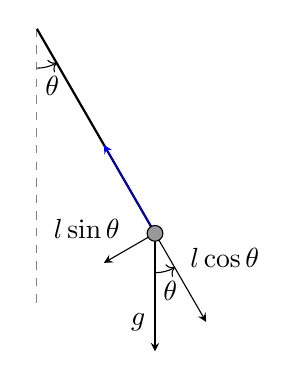
\begin{tikzpicture}
			\pgfmathsetmacro{\Gvec}{1.5}
			\pgfmathsetmacro{\myAngle}{30}
			% calculate lengths of vector components
			\pgfmathsetmacro{\Gcos}{\Gvec*cos(\myAngle)}
			\pgfmathsetmacro{\Gsin}{\Gvec*sin(\myAngle)}
			
			\coordinate (centro) at (0,0);
			\draw[dashed,gray,-] (centro) -- ++ (0,-3.5) node (mary) [black,below]{$ $};
			\draw[thick] (centro) -- ++(270+\myAngle:3) coordinate (bob);
			\pic [draw, ->, "$\theta$", angle eccentricity=1.5] {angle = mary--centro--bob};
			\draw [blue,-stealth] (bob) -- ($(bob)!\Gcos cm!(centro)$);
			\draw [-stealth] (bob) -- ($(bob)!-\Gcos cm!(centro)$)
			coordinate (gcos)
			node[midway,above right] {$l\cos\theta$};
			\draw [-stealth] (bob) -- ($(bob)!\Gsin cm!90:(centro)$)
			coordinate (gsin)
			node[midway,above left] {$l\sin\theta$};
			\draw [-stealth] (bob) -- ++(0,-\Gvec)
			coordinate (g)
			node[near end,left] {$g$};
			\pic [draw, ->, "$\theta$", angle eccentricity=1.5] {angle = g--bob--gcos};
			\filldraw [fill=black!40,draw=black] (bob) circle[radius=0.1];
			\end{tikzpicture}
		\end{center}
		\caption{Péndulo en $ℝ^n$}
	\end{wrapfigure}
	
	Supongamos que queremos ver el movimiento de un péndulo. En lugar de imaginar fuerzas y tensiones ficticias, veámoslo matemáticamente. El punto extremo del péndulo tiene coordenadas $(x,y)$ y entonces $L=\frac{1}{2}m(\dot{x}^2+\dot{y}^2)-mgy$. Si nos fijamos, $(x,y)$ no son buenas coordenadas para este problema. Cojamos mejor la coordenada $\theta=$ángulo. Entonces$$ \begin{cases}
		x=l\cdot sen(\theta)\\
		y=-l\cdot cos(\theta)\\
	\end{cases}\longrightarrow \begin{cases}
	dx=l\cdot cos(\theta)d\theta\\
	dy=-l\cdot cos(\theta)d\theta\\
	\end{cases}$$
	y entonces $L=\frac{1}{2}m\cdot l^2\dot{\theta}^2+mgl\cdot cos(\theta)$. \\Ahora aplicando \refeq{eq:Euler-Lagrange} tenemos:
	$$\dv{t}\left(\pdv{L}{\dot{\theta}}\right)=\pdv{L}{\theta}\longrightarrow\dv{t}\left(ml^2\dot{\theta}\right)=-mgl\cdot sen(\theta)\longrightarrow\ddot{\theta}=-\frac{g}{l}sen(\theta)$$
	que es la ecuación del péndulo de toda la vida.
\end{example}
\\
\begin{obs}
	Este resultado de invarianza ante cambios de coordenadas  nos llevará como veremos a calcular geodésicas en variedades muy rápidamente si lo vemos como un problema del cálculo de variaciones minimizando las métricas en dicha variedad.
\end{obs}
\section{Geodésicas en variedades}
\begin{defn}[Variedad\IS semiriemanniana] Una variedad semiriemanniana es una variedad dotada de una métrica.
\end{defn}

\begin{defn}[Variedad\IS riemanniana] Una variedad riemanniana es una variedad semiriemanniana cuya métrica es definida positiva.
\end{defn}

Recuérdese que la condición de no degeneración que se pedía a una métrica G es que su matriz de componentes ($g_{ij}$) fuera no singular. Esto no impide que ocurran cosas raras como $G(∂1, ∂1) = 0$  o $G(∂1, ∂1) < 0$. Tal comportamiento estrafalario (¿vectores con longitudes nulas o imaginarias?) es conveniente en relatividad pero extraño a nuestras ideas geométricas, por ello es natural dar una denominación específica a las variedades con métricas definidas positivas, es decir, con matriz ($g_{ij}$) definida positiva en todo punto.\newline
****FALTA UN DIA DE CLASE AQUI****\newline
Lo último que habíamos visto es que si teníamos una geodésica entonces estaba parametrizada por arco cumpliendo $g_{ij}\dot{x}^i\dot{x}^j=cte$.
Los símbolos de Christoffel son algo que aparece de manera natural al estudiar la geometría de superficies de forma extrínseca (fijándose en el entorno). La curvatura se suele calcular usando el producto de curvaturas principales (extrínsecamente) o con formas diferenciables (intrínsecamente).

Sobre los símbolos de Christoffel: Si la matriz $(g_{ij})$ era definida positiva yo puedo reparametrizar la curva: $$x^i(t)\longrightarrow x^i(kt); \text{ luego tenemos que } \dv{t}(x^i(kt))=k\dot{x}^i(kt)\text{ y por tanto:}$$$$ g_{ij}\dot{x}^i\dot{x}^j=cte\longrightarrow  k^2g_{ij}\dot{x}^i\dot{x}^j=cte$$
Tomando $k^2=cte$ conseguiría $g_{ij}\dot{x}^i\dot{x}^j=1$. Esto es porque la constante es positiva (porque la matriz es definida positiva), en otro caso no puedo parametrizar por longitud de arco todas las geodésicas (no sería igual a 1).
\begin{obs}Recordemos que para poder parametrizar por longitud de arco tenemos que tener $G(\overline{v},\overline{v})=1$, que es lo mismo que se ve en GCS.
\end{obs}

Vamos a atar algunos cambios sueltos, como que no está claro que estén "bien" definidas las geodésicas. Sabemos que funcionan con cambio de carta (aunque no lo hemos visto con todo rigor), pero ¿funcionan como en GCS que dado un valor inicial y un vector inicial ya tengo definida una sola geodésica? ¿Nos salen las mismas geodésicas que en segundo? ¿minimizan las geodésicas la longitud en pequeños entornos?.\\ \indent Sabemos que algunas EDO tienen más de una solución así que \textbf{no está claro} que estén bien definidas (especialmente en los casos que no hay unicidad o existencia de la EDO asociada). \\ \indent Desde el punto de vista de la física la primera y la última pregunta se contestan fácil: Por ejemplo, dada una partícula si le pones una posición inicial y un vector inicial está definida si miramos el momento y el espacio donde está, luego la respuesta sería que sí, que está bien definida (por tramposo que parezca el razonamiento). Por otro lado, por el principio de mínima acción también nos haría intuir una respuesta afirmativa.\\
\begin{wrapfigure}{r}{0.3\textwidth}
	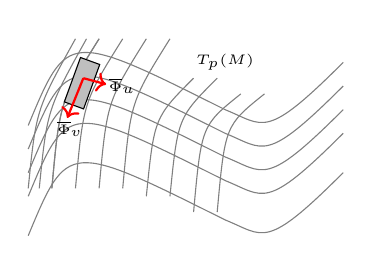
\begin{tikzpicture}[remember picture]   
	%horizantal
	\foreach \y in {0.6, 0.9, 1.2, 1.5}
	\draw[xshift=0.2cm , yshift=\y cm, gray] (-2,-1.8)..controls (-1.5,-0.6)..(0.5,-1.6)
	(0.5,-1.6)..controls (1.0,-1.8) and (1,-2)..(2,-1);
	\draw[xshift=0.2cm , yshift=0.1cm, gray] (-2,-1.8)..controls (-1.5,-0.6)..(0.5,-1.6)
	(0.5,-1.6)..controls (1.0,-1.8) and (1,-2)..(2,-1);
	%vertical                                                 
	\draw[xshift=0.1 cm , yshift=-0.0cm, gray]     (-1.9,-1.1)..controls (-1.8,-0.1)..(-1.3,0.8);                                
	\draw[xshift=0.24 cm , yshift=-0.0cm,gray]     (-1.9,-1.1)..controls (-1.8,-0.1)..(-1.3,0.8);                           
	\draw[xshift=0.4 cm , yshift=-0.0cm, gray]     (-1.9,-1.1)..controls (-1.8,0)..(-1.3,0.8);                                               
	\foreach \x in { 0.4, 0.7, 1.0, 1.3}             
	\draw[xshift=\x cm , yshift=-0.0cm, gray]     (-1.9,-1.1)..controls (-1.8,0)..(-1.3,0.8);
	\foreach \x in { 1.6, 1.9}             
	\draw[xshift=\x cm , yshift=-0.3cm,gray]      (-1.9,-0.9)..controls (-1.8,0.1)..(-1.3,0.6);
	\foreach \x in { 2.2, 2.5}             
	\draw[xshift=\x cm , yshift=-0.3cm, gray]     (-1.9,-1.1)..controls (-1.8,0)..(-1.3,0.4);
	%rectangle
	\draw [rectangle,fill=gray!50,rotate=-20,xshift=-1.13cm,yshift=-0.16cm](-0.13,-0.3) rectangle (0.13,0.3);
	\node[](nodeA) at (-1.1cm,0.4cm){};
	\node[black](nodeB) at (0.7cm,0.5cm) {\tiny{$T_p(M)$}};
	%coord syst
	\draw [->,thick,color=red,xshift=-1.1cm,yshift=0.3cm,rotate=-15](0,0) -- (xyz cs:x=0.3) ; 
	\node [black, above, xshift=-1cm,yshift=-0.6cm] at (-0.2,1.3) {\tiny{}};  
	%\draw [->,thick,color=red, xshift=-1.1cm,yshift=0.3cm,rotate=10](0,0) -- (xyz cs:y=0.5) ;
	\node [black, right, xshift=-1.8cm] at (0.9,0.2) {\tiny{$\overline{\Phi}_u$}};
	\draw [->,thick,color=red, xshift=-1.1cm,yshift=0.3cm,rotate=23](0,0) -- (xyz cs:z=1.0) ; 
	\node [black, above, xshift=-0.67cm,yshift=0.3cm] at (-0.6,-0.87) {\tiny{$\overline{\Phi}_v$}};     
	\end{tikzpicture}
	\Varrow{black}{nodeA}{nodeB}         
\end{wrapfigure}
\indent Vamos a dar demostraciones matemáticas para dejar de intuír. En Geometría de Curvas y Superficies, se trabaja con el siguiente sistema de referencia: $\{\overline{\Phi}_u,\overline{\Phi}_v,\overline{N}\}$ .\\ \indent Con este criterio cada vector de $\mathbb{R}^3$ tendrá unas componentes en esta base.Si no sabemos que la superficie está en $\mathbb{R}^3$ se usan los símbolos de Christoffel, dando las componentes en $\overline{\Phi}_u,\overline{\Phi}_v$ de sus derivadas.\\
\indent Cuando uno calcula la aceleración de una partícula en $\overline{\Phi}_u$ tenemos $$\pdv[2]{\overline{\Phi}}{u}=\overline{\Phi}_{uu}=\Gamma^1_{11}\overline{\Phi}_u+\Gamma^2_{11}\overline{\Phi}_v+e\overline{N}$$, donde e es el primer coeficiente de la 2ª forma fundamental. Lo mismo con las otras derivadas $\overline{\Phi}_{uv}$ y $\overline{\Phi}_{vv}$. Los símbolos de Christoffel son las $\Gamma$. Estos símbolos se usan porque las curvaturas en realidad sólo dependen de las métricas: la curvatura de Gauss se puede dar en función de $e,f,g$ (coeficientes de la $II FF$), pero haciendo magia negra podemos dejarla en función sólo de los símbolos de Christoffel, convirtiéndose esta en un invariante intrínseco de la variedad (\textbf{theorema egregium} de Gauss).
\begin{prop}
Las ecuaciones de Euler-Lagrange que definen las geodésicas son equivalentes a estas con una pinta más amable
\begin{equation}
\ddot{x}^k+\Gamma^k_{ij}\dot{x}^i\dot{x}^j=0
\end{equation}
donde los $\Gamma^k_{ij}$ son los simbolos de Christoffel dados por esta difícil expresión
\begin{equation}
\Gamma^k_{ij}=\frac{1}{2}g^{mk}\left(\pdv{g_{im}}{x^j}+\pdv{g_{jm}}{x^i}-\pdv{g_{ij}}{x^m}\right)
\end{equation}
con $(g^{ij})$ la matriz inversa de $(g_{ij})$. En particular, existe una única geodésica una vez escogidos punto y vector inicial $x^i(0)$ y $\dot{x}^i(0)$. Si $(g_{ij})$ es una métrica como es no singular se puede calcular la inversa, y como las funciones serán $C^\infty$ todo se podrá calcular.
\end{prop}
\begin{obs} Esta proposición se usa para calcular los símbolos de Christoffel en casos sencillos (pocas dimensiones y métricas sencillas) sin usar la fórmula, simplemente hallando las ecuaciones diferenciales de las geodésicas y comparar coeficientes.
\end{obs}
\begin{example} Hallaremos los símbolos de Christoffel para $\mathbb{S}^2$ con la métrica inducida y la carta $(\theta,\phi)$.
Sabíamos que la métrica es $G=d\theta^2+sen^2(\theta)d\phi^2$, habíamos hallado las ecuaciones de Euler-Lagrange de las geodésicas y teníamos, con lagrangiano $L=\dot{\theta}^2+sen^2(\theta)\dot{\phi}^2$: $$\dv{t}\left(\pdv{L}{\dot{\theta}}\right)=\pdv{L}{\theta}\longrightarrow\ddot{\theta}=2sen(\theta)cos(\theta)\dot{\phi}^2\longrightarrow\ddot{\theta}-sen(\theta)cos(\theta)\dot{\phi}^2=0\longrightarrow\ddot{x}^1+\Gamma^1_{ij}\dot{x}^i\dot{x}^j=0$$
$$\Gamma^1_{22}=-sen(\theta)cos(\theta)$$ y el resto son 0. Por otro lado:
$$\dv{t}\left(\pdv{L}{\dot{\phi}}\right)=\pdv{L}{\phi}\longrightarrow\dv{t}(2sen^2(\theta)\dot{\phi})=0\longrightarrow4sen(\theta)cos(\theta)\dot{\theta}\dot{\phi}+2sen^2(\theta)\ddot{\phi}=0;$$$$\ddot{\phi}+2\frac{cos(\theta)}{sen(\theta)}\dot{\theta}\dot{\phi}=0\longrightarrow\ddot{x}^2+\Gamma^2_{ij}\dot{x}^i\dot{x}^j=0\longrightarrow\begin{cases}
\Gamma^2_{12}=\Gamma^2_{21}=\frac{cos(\theta)}{sen(\theta)}\\
\Gamma^2_{ij}=0 \text{ en otro caso}\\
\end{cases}$$
\end{example}
\begin{prop}Las geodésicas en una variedad satisfacen las siguientes ecuaciones:
\begin{equation}
\ddot{x}^i+\Gamma^i_{jk}\dot{x}^i\dot{x}^j=0
\end{equation}
donde $\Gamma^i_{jk}$ don los símbolos de Christoffel.
\end{prop}
\begin{proof} A partir de la k-ésima ecuación de Euler-Lagrange tenemos: $$\dv{t}(2g_{kj}\dot{x}^j)=2\pdv{g_{ij}}{x^k}\dot{x}^i\dot{x}^j;$$
	$$2g_{kj}\ddot{x}^j-\pdv{g_{ij}}{x^k}\dot{x}^i\dot{x}^j=-2\pdv{g_{kj}}{x^i}\dot{x}^i\dot{x}^j=\left(-\pdv{g_{kj}}{x^i}-\pdv{g_{ki}}{x^j}\right)\dot{x}^i\dot{x}^j;$$$$g_{kj}\ddot{x}^j+\frac{1}{2}\left(\pdv{g_{kj}}{x^i}+\pdv{g_{ki}}{x^j}-\pdv{g_{ij}}{x^k}\right)\dot{x}^i\dot{x}^j=0;$$
	Sabemos que $g_{kj}\ddot{x}^j$ se corresponde a coger la k-ésima coordenada del producto matricial $\begin{pmatrix}g_{11}&\cdots&g_{1n}\\\vdots&\ddots&\vdots\\g_{n1}&\cdots&g_{nn}\\\end{pmatrix}\begin{pmatrix}\ddot{x}^1\\\vdots\\\ddot{x}^n\end{pmatrix}$ Si ahora multiplicamos por la matriz inversa se tiene $g^{lk}g_{kj}\ddot{x}^j=\delta^l_j\ddot{x}^j=\ddot{x}^l$ y ya sale la fórmula con los símbolos de Christoffel
\end{proof}
En las variedades no se tiene en cuenta el vector normal $\overline{N}$, de hecho para dimensiones grandes no existe la segunda forma fundamental, mientras que los símbolos de Christoffel existen en cualquier variedad.
\subsection{Relatividad General}
La teoría de la relatividad general, postulada por Albert Einstein, es en realidad bastante geométrica. Einstein postuló (a grandes rasgos) que el potencial gravitatorio (o fuerza de la gravedad) no existía (es decir, que toda la energía de las partículas era energía cinética), y a cambio de esto, la energía cinética viene reemplazada por una métrica (que él no calculó). Einstein sólo sabía de dicha métrica las condiciones complicadísimas que debía cumplir, (esencialmente que la curvatura fuese nula en algún sentido), pero no la formuló.

\indent Con esta filosofía, las trayetorias de las partículas materiales serán las geodésicas parametrizadas por longitud de arco ($G(\dot{\gamma},\dot{\gamma})=1$), siendo el parámetro de las geodésicas el tiempo medido por un observador en la partícula.
Para las trayectorias de las partículas de luz tenemos que serán las geodésicas que cumplen ($G(\dot{\gamma},\dot{\gamma})=0$).
\begin{example}Para movimientos radiales (como la caída de una piedra al centro de la tierra) bajo el efecto de una masa m con simetría esférica que no esté rotando (estática), la métrica fuera de ella es la \textbf{Métrica de Schwarzchild (radial)} (que ya apareció antes en estas notas como la métrica alrededor de un agujero negro):
	$$G=\left(1-\frac{r_0}{r}\right)dt^2-c^{-2}\left(1-\frac{r_0}{r}\right)^{-1}dr^2$$
donde c es la velocidad de la luz, r es la distancia al centro y $r_0$ una constante dada por $r_0=\frac{2gm}{c^2}$ donde g es la constante de gravitación y m como ya dijimos la masa.\\ \indent En $r=r_0$ la matriz de la métrica se vuelve singular (aparecen un coeficiente 0 en la coordenada temporal y un $\infty$ en la espacial) y el asunto se pone feo (aparece una especie de potencial gravitatorio infinito).\\ \indent En el caso de los planetas, estrellas, etc. el valor de $r_0$ es muy pequeño con respecto al radio del cuerpo en cuestión (en el caso de La Tierra tenemos $r_0\approx8mm$). Existen sin embargo objetos llamados agujeros negros, que son unas "estrellas raras" con radio menor que $r_0$, es decir, que la singularidad queda fuera.\\ \indent Vamos a calcular ahora las geodésicas más sencillas (correspondientes a un rayo de luz) para esta métrica. Para ello recordemos que se tenía que cumplir $G(\dot{\gamma},\dot{\gamma})=0$ y vamos a ver como solo usando \ref{eq:ConservacionEnergia} podemos ver la forma de las geodésicas:
$$\left(1-\frac{r_0}{r}\right)dt^2-c^{-2}\left(1-\frac{r_0}{r}\right)^{-1}dr^2=0\tab\begin{cases}t=t(\lambda);\\r=r(\lambda);\end{cases}\begin{cases}\dot{t}=\dv{t}{\lambda};\\\dot{r}=\dv{r}{\lambda};\end{cases}\frac{\dot{t}}{\dot{r}}=\frac{dt}{dr}$$ 
\indent Por la conservación de la energía, si la métrica es 0 en el instante inicial entonces es 0 siempre.
$$\left(\dv{t}{r}\right)^2=c^{-2}\left(1-\frac{r_0}{r}\right)^{-2}\xrightarrow{\textbf{quitamos} \sqrt{}}\dv{t}{r}=\pm c^{-1}\left(1-\frac{r_0}{r}\right)^{-1}$$
Ya tenemos la EDO que satisfacen las geodésicas, que encima es de variables separadas, así que tomando $\int_{r_o}^{r}$:
$$t=\pm c^{-1}\restr{(r+r_0\log(r-r_0))}{R_0}^R;$$
$$\pm ct=r-R_0+r_0\log(\frac{r-r_0}{R_0-r_0});$$
Luego si el rayo se acerca al agujero negro tenemos $R=R_0$ sale un $\infty$ (esto significa que, visto desde fuera, cuando el rayo de luz va acercándose al agujero negro, tarda un "tiempo infinito" en atravesarlo, es decir, lo vemos parado).
\end{example}


%% Apéndices (ejercicios, exámenes)
\appendix

\chapter{Ejercicios}
% -*- root: ../GeoTopo17.tex -*-
\section{Hoja 1}
\begin{problem}[1]Responde brevemente a las siguientes preguntas:
	\ppart Si $T=T(\overline{x},\overline{y})$ y $S=S(\overline{x},\overline{y})$ son tensores, ¿lo es $T(\overline{x},\overline{y})\cdot S(\overline{x},\overline{y})$?¿y $T(\overline{x},\overline{y})+S(\overline{x},\overline{y})$?
	\ppart ¿Es $T(\overline{x},\overline{y})=\overline{x}+\overline{y}$ una aplicación bilineal?
	\ppart ¿Cuántas componentes tiene un tensor (r,s) con $V=ℝ^{m}$?
	\ppart ¿Es un tensor la aplicación que dados dos vectores de $ℝ^{3}$ les asigna la primera coordenada de su producto vectorial?
	\ppart ¿Es un tensor la aplicación que a cada par de vectores de $ℝ^{2}$ con la base canónica les asigna el área del paralelogramo que determinan?
	
	\solution
	\textit{Hecho por Jose, se aceptan correcciones}\\
	\spart Tenemos $$\appl{T}{ℝ^{n}×ℝ^{n}}{ℝ};\tab\appl{S}{ℝ^{n}×ℝ^{n}}{ℝ};\tab\text{ambos multilineales}$$\indent Es fácil observar que $T\cdot S(\overline{x},\overline{y})=T(\overline{x},\overline{y})\cdot S(\overline{x},\overline{y})$ no es multilineal , ya que $$T\cdot S(\alpha\cdot\overline{x},\overline{y})=\alpha^2\cdot T\cdot S(\overline{x},\overline{y})$$ \indent luego no es tensor.\newline
	\indent Si ahora nos fijamos en $T+S(\overline{x},\overline{y})=T(\overline{x},\overline{y})+S(\overline{x},\overline{y})$ es inmediato comprobar que es \indent un tensor 2 veces covariante:
	$$T+S(\alpha\cdot\overline{x},\overline{y})=T(\alpha\overline{x},\overline{y})+S(\alpha\overline{x},\overline{y})=\alpha\cdot(T+S(\overline{x},\overline{y}))$$
	$$T+S(\overline{x}_1+\overline{x}_2,\overline{y})=T(\overline{x}_1,\overline{y})+S(\overline{x}_1,\overline{y})+T(\overline{x}_2,\overline{y})+S(\overline{x}_2,\overline{y})=(T+S(\overline{x}_1,\overline{y}))+(T+S(\overline{x}_2,\overline{y}))$$
	\spart \indent Inmediato comprobar que no es bilineal multiplicando una variable por un escalar: $$T(\alpha\overline{x},\overline{y})=\alpha\overline{x}+\overline{y}\neq\alpha(\overline{x}+\overline{y})$$
	\newpage
	\spart $$\appl{T}{\underbrace{(ℝ^{m})^{*}×\cdots×(ℝ^{m})^{*}}_{\text{r veces}}×\underbrace{ℝ^{m}×\cdots×ℝ^{m}}_{\text{s veces}}}{ℝ}$$ \indent luego habrá $m^{r+s}$ componentes.
	
	\spart  Hay dos formas, una es considerar:
	\begin{align*}
		\appl{T}{ℝ^{3}×ℝ^{3}&}{ℝ} \\
		T\left(\begin{pmatrix}x_1\\x_2\\x_3\end{pmatrix},\begin{pmatrix}y_1\\y_2\\y_3\end{pmatrix}\right) &\longmapsto{x_2\cdot y_3-x_3\cdot y_2}
	\end{align*}
 	y comprobar que efectivamente se cumplen las condiciones de multilinealidad. \\
 	La segunda es considerar:
 	\begin{align*}
 		\appl{T}{ℝ^{3}×ℝ^{3}&}{ℝ} \\
 		T\left(\begin{pmatrix}x_1\\x_2\\x_3\end{pmatrix},\begin{pmatrix}y_1\\y_2\\y_3\end{pmatrix}\right) &\longmapsto{(\overline{x}×\overline{y})\cdot\overline{e}_1=\begin{vmatrix}
 				1 & 0 &  0 \\ 
 				x_1 & x_2 & x_3 \\ 
 				y_1 & y_2 & y_3 \\ 
 		\end{vmatrix}}
 	\end{align*}
	y como vimos que el determinante es multilineal, pues ya está demostrado porque es un determinante.
	
	\spart 
		\begin{align*}
		\appl{T}{ℝ^{2}×ℝ^{2}&}{ℝ} \\
		T(\overline{x},\overline{y}) &\longmapsto{A=\text{área}}
	\end{align*}
\indent El área siempre es $\geq 0$, luego si multiplico por $\lambda=-1$ tenemos $T(\lambda\overline{x},\overline{y})\neq\lambda T(\overline{x},\overline{y})$
	
\end{problem}
\begin{problem}[2] Demuestra que, fijada una base, todo tensor dos veces covariante es de la forma $T(\overline{x},\overline{y})=\overline{x}^TA\overline{y}$ con A una matriz cuadrada.
	
	\solution Tenemos una base cualquiera, luego si llamamos $\overline{e}_i$ a los vectores de dicha base tenemos que $\overline{x}$,$\overline{y}$ son de la forma $\begin{cases}\overline{x}=x^i\overline{e}_i\\\overline{y}=y^i\overline{e}_i\end{cases}$ y por tanto tenemos: $$T(\overline{x},\overline{y})=x^iy^j\underbrace{T(\overline{e}_i,\overline{e}_j)}_{a_{ij}}=x^ia_{ij}y^j=\begin{pmatrix}x^1&\cdots&x^n\end{pmatrix}\begin{pmatrix}a_{11}&\cdots&a_{1n}\\\vdots&\ddots&\vdots\\a_{n1}&\cdots&a_{nn}\end{pmatrix}\begin{pmatrix}y^1\\\vdots\\y^n\end{pmatrix}\qed$$
\end{problem}
\begin{problem}[3] Halla cuántas componentes nulas y cuántas componentes no nulas tiene el tensor determinante en $ℝ^{n}$. Estudia cuántas son positivas.
	
	\solution \textit{Hecho por Jose, se aceptan correcciones}\\
	Sea el tensor n veces covariante en $ℝ^{n}$ y la base canónica $\base = \{ \overline{e}_1,...,\overline{e}_n \}$ de $ℝ^{n}$:
	
\begin{align*}
	\appl{D}{\underbrace{(ℝ^{n})×\cdots×(ℝ^{n})}_{\text{n veces}}&}{ℝ} \\
	D(\overline{x}_1,\cdots,\overline{x}_n) &\longmapsto{\begin{vmatrix}
							\overline{x}_1 & \cdots &  \overline{x}_n \\ 
						\end{vmatrix}}
\end{align*}
		El tensor tienen $n^n$ componentes:
		$$D_{1\space1\cdots1}=\begin{vmatrix}
		1 & 1 &\cdots & 1 \\ 
		0& 0 &\cdots & 0 \\ 
		\vdots & \vdots &\ddots & \vdots \\ 
		0& 0 &\cdots & 0 \\ 
		\end{vmatrix}$$
	En cuanto el determinante contenga a dos $\overline{e}_i$ que tengan la misma $i$ ya da 0 (por ser determinante de elementos linealmente dependientes). Luego para que no sea nulo ha de tener todas los índices distintos. Esto nos dice que el número de componentes no nulas son las permutaciones de $n$ elementos ($n!$), y las nulas serían entonces $n^n - n!$.\\
	Ahora, de las que no son nulas vamos a ver cuales son positivas. Probando descubrimos que con esta base hay dos valores posibles del determinante que son $1$ y $-1$. Las componentes positivas son aquellas que valen $1$ y esto ocurre cuando hay un número par de $\overline{e}_i$ cambiadas de posición (recordemos que todas las $i$ son ahora distintas porque estamos en el caso no nulo). \\
	La conclusión es que la cantidad de las que valen $1$ es la cantidad de permutaciones pares de n elementos, que es $\frac{n!}{2}$.
\end{problem}\newpage
\begin{problem}[4] \ppart Si multiplicamos tensorialmente unos cuantos elementos de $\mathcal{B}$ y otros de $\mathcal{B}^*$, halla cuántas componentes no nulas tiene el tensor resultante. Explica por qué todo tensor se puede escribir como combinación lineal de estos productos tensoriales y \ppart hazlo para el tensor que corresponde a la rotación de ángulo $\frac{\pi}{2}$ escogiendo $\mathcal{B}=\{\overline{e}_1+\overline{e}_2,\overline{e}_2\}$ siendo los $\overline{e}_i$ los vectores canónicos habituales.
	
	\solution \textit{Hecho por Jose, se aceptan correcciones}\\ \spart Sean $\mathcal{B}=\{\overline{e}_1,\cdots\overline{e}_n\}$ y $\mathcal{B}^*=\{\tilde{\phi}^1,\cdots\tilde{\phi}^n\}$ donde los $\overline{e}_i$ son tensores de tipo (1,0) y los $\tilde{\phi}^i$ son tensores de tipo (0,1). Tenemos. por la propiedad de la base dual, que $$\overline{e}_i(\tilde{\phi^{j}})=\tilde{\phi}^j(\overline{e}_i)=\delta^i_j=\begin{cases}0\tab i\neq j\\1\tab i=j
	\end{cases}$$ Si cogemos ahora $m$ de esos tensores $(1,0)$ y k de esos tensores $(0,1)$ y los multiplicamos tensorialmente, por definición nos queda un tensor de tipo $(m,k)$ cuyas componentes son:	$$\overline{e}_{i_1}\otimes\cdots\otimes\overline{e}_{i_m}\otimes\tilde{\phi^{j_1}}\otimes\cdots\otimes\tilde{\phi^{j_k}}(\tilde{\phi^{s_1}},\cdots,\tilde{\phi^{s_m}},\overline{e}_{r_1},\cdots,\overline{e}_{r_k})=\overline{e}_{i_1}(\tilde{\phi^{s_1}})\cdots\overline{e}_{i_m}(\tilde{\phi^{s_m}})\cdot\tilde{\phi^{j_1}}(\overline{e}_{r_1})\cdots\tilde{\phi^{j_k}}(\overline{e}_{r_k})=$$ $$=\delta_{i_1}^{s_1}\cdots\delta_{i_m}^{s_m}\cdot\delta_{j_1}^{r_1}\cdots\delta_{j_k}^{r_k}=\begin{cases}1\tab \text{si los }\delta^A_B\text{ valen todos 1}\\0\tab \text{en otro caso}
	\end{cases}$$
	La descomposición es de la siguiente manera:
	$$T(\tilde{x}^1,\cdots,\tilde{x}^m,\overline{y}_1,\cdots,\overline{y}_k)=T(x^1_{i_1}\phi^{i_1},\cdots,x^m_{i_m}\phi^{i_m},\overline{y}_1^{j_1}\overline{e}_{j_1},\cdots,\overline{y}_k^{j_k}\overline{e}_{j_k})=x^i_{i_1}\cdots x^m_{i_m}y_1^{j_1}\cdots y_k^{j_k};$$
	$$T^{i_1\cdots i_m}_{j_1\cdots j_k}=x^1_{h_1}\delta^{h_1}_{i_1}\cdots x^m_{h_m}\delta^{h_m}_{i_m}y_1^{h_1}\delta^{j_1}_{h_1}\cdots y_k^{h_k}\delta^{j_k}_{h_k};$$
	\spart Tenemos una aplicación lineal, luego se corresponde unívocamente con un tensor $G$ de tipo $(1,1)$, y siendo $f(\overline{x})$ la aplicación lineal con matriz $A$ en dicha base aplicada a $\overline{x}$:
	\begin{align*}
	\appl{G}{(ℝ^2)^*×ℝ^2&}{ℝ} \\
	G(\tilde{\phi},\overline{x}) &\longmapsto{\tilde{\phi}(f(\overline{x}))=\tilde{\phi}(A(\overline{x}))}
	\end{align*}
	Tenemos la base $\mathcal{B}_R=\{\overline{e}_1+\overline{e}_2,\overline{e}_2\}=\{\begin{pmatrix}1\\1\end{pmatrix},\begin{pmatrix}0\\1\end{pmatrix}\}$, buscamos su base dual y tenemos $\mathcal{B}^*_R=\{\begin{pmatrix}1&0\end{pmatrix},\begin{pmatrix}-1&1\end{pmatrix}\}$.\\
	Ahora, aplicando a los elementos de la base por el giro sabemos que $A\cdot(\overline{e}_1+\overline{e}_2)=-\overline{e}_1+\overline{e}_2$ y que $A\cdot\overline{e}_2=-\overline{e}_1$ y calculamos las componentes:$$\begin{cases}
	T(\tilde{\phi^{1}},\overline{e}_1+\overline{e}_2)=\tilde{\phi^{1}}(A\cdot(\overline{e}_1+\overline{e}_2))=-1\\
	T(\tilde{\phi^{1}},\overline{e}_2)=-1\\
	T(\tilde{\phi^{2}},\overline{e}_1+\overline{e}_2)=2\\
	T(\tilde{\phi^{2}},\overline{e}_2)=1
	\end{cases}$$\newpage
	Ahora sabemos que como es un tensor tipo $(1,1)$ se puede escribir como producto tensorial de un tensor $(1,0)$ (fijando un vector $\overline{v}_1$) y otro $(0,1)$ (fijando un elemento del dual $\tilde{\phi}^1$):
\begin{align*}
	\appl{T}{V^*&}{ℝ}&\appl{S}{V&}{ℝ}\\
	T(\tilde{\phi}) &\longmapsto{\tilde{\phi}(\overline{v}_1)}&S(\overline{v}) &\longmapsto{\tilde{\phi}^1(\overline{v})}
\end{align*}
\begin{align*}
	\appl{T\otimes S}{V^*×V&}{ℝ} \\
	T\otimes S(\tilde{\phi},\overline{v}) &\longmapsto{\tilde{\phi}(\overline{v}_1)\cdot\tilde{\phi}^1(\overline{v})}
\end{align*}
\end{problem}
\begin{problem}[5] Para $V=ℝ^3$ consideremos un tensor de tipo $(0,3)$, otro de tipo $(1,2)$ y otro de tipo $(2,1)$, cuyas componentes, digamos $\epsilon_{ijk}$, $\epsilon^i_{jk}$ y $\epsilon^{ij}_k$ en la base canónica son: 0 si $i,j,k$ no es una reordenación de $1,2,3$; 1 si  $i,j,k$ es una permutación par de $1,2,3$ y -1 si  $i,j,k$ es una permutación impar de $1,2,3$. Dados $\overline{u},\overline{v},\overline{w}\inℝ^3$ y $\overline{F}=(F^1,F^2,F^3)$, explica qué objetos matemáticos bien reconocidos representan las siguientes cantidades: $\epsilon^{ij}_k\pdv{F^k}{x^j}$,$\epsilon^i_{jk}v^jw^k$ y $\epsilon_{ijk}u^iv^jw^k$
	\solution \textit{Hecho por Jose, se aceptan correcciones}\\ \begin{wraptable}{l}{5.5cm}
	\begin{tabular}{| c | c | c | c | c |}
		\hline
		TIPO & i & j & k & VALOR\\ \hline
		par & 1 & 2 & 3 & 1\\ \hline
		impar & 1 & 3 & 2  & -1\\ \hline
		par & 2 & 3 & 1 & 1\\ \hline
		impar & 2 & 1 & 3 & -1\\ \hline
		par & 3 & 2 & 1  & 1\\ \hline
		impar & 3 & 1 & 2 & -1\\ \hline
	\end{tabular}
\end{wraptable}
En primer lugar vemos que los tensores tienen $3^3=27$ componentes, pero de ellas solo tenemos que no son nulas las reordenaciones de $(1,2,3)$, que son $3!=6$ componentes no nulas con valores dependiendo de la permutación como se ve en la tabla. Conociendo ahora los valores de cada componente y recordando el criterio de Einstein vamos a ver caso a caso de qué pueden tratar esas expresiones:\\
\begin{itemize}
	\item $\epsilon^{ij}_k\pdv{F^k}{x^j}=(\pdv{F^3}{x^2}-\pdv{F^2}{x^3},\pdv{F^1}{x^3}-\pdv{F^3}{x^1},\pdv{F^2}{x^1}-\pdv{F^1}{x^2})=\begin{vmatrix}
	\overline{e}_1 & \overline{e}_2 &  \overline{e}_3 \\ 
	\pdv{x^1} & \pdv{x^2} & \pdv{x^3} \\ 
	F^1 & F^2 & F^3 \\ 
	\end{vmatrix}=\overline{rot}(\overline{F})$
	\item $\epsilon^i_{jk}v^jw^k=(v^2w^3-v^3w^2,v^3w^1-v^1w^3,v^1w^2-v^2w^1)=\begin{vmatrix}
	\overline{e}_1 & \overline{e}_2 &  \overline{e}_3 \\ 
	v^1 & v^2 & v^3 \\ 
	w^1 & w^2 & w^3 \\ 
	\end{vmatrix}=\overline{v}×\overline{w}$
	\item $\epsilon_{ijk}u^iv^jw^k=u^1(v^2w^3-v^3w^2)-u^2(v^1w^3-v^3w^1)+u^3(v^1w^2-v^2w^1)=\begin{vmatrix}
	u^1 & u^2 &  u^3 \\ 
	v^1 & v^2 & v^3 \\ 
	w^1 & w^2 & w^3 \\ 
	\end{vmatrix}=\overline{u}\cdot(\overline{v}×\overline{w})$
\end{itemize}
\newpage
\end{problem}
\begin{problem}[6] Demuestra que el "tensor identidad" $\appl{T_{\text{id}}}{(ℝ^2)^*×ℝ^2}{ℝ}$ que tiene componentes $\delta_j^i$ en la base canónica conserva las componentes en cualquier otra base.
	\solution \textit{Hecho por Jose, se aceptan correcciones}\\ Estamos en $(ℝ^2)^*×ℝ^2$. Tenemos las bases canónicas $\mathcal{B}=\{\overline{e}_1,\overline{e}_2\}$, $\mathcal{B^*}=\{\tilde{\phi}^1,\tilde{\phi}^2\}$ y el tensor definido como:
		\begin{align*}
		\appl{T}{(ℝ^2)^*×ℝ^2&}{ℝ} \\
		T(\tilde{\phi},\overline{x}) &\longmapsto{\tilde{\phi}f(\overline{x})=\tilde{\phi}A\overline{x}}
	\end{align*}
donde en este caso, como $f$ es la identidad, tenemos que $A$ es la matriz identidad y nos queda:
\begin{align*}
	\appl{T}{(ℝ^2)^*×ℝ^2&}{ℝ} \\
	T(\tilde{\phi},\overline{x}) &\longmapsto{\tilde{\phi}\overline{x}}
\end{align*}
Es claro comprobar que las componentes de $T$ se corresponden con las $\delta_j^i$ (recordar la propiedad de la base dual). Si cambiamos de bases, digamos a otras $\tilde{\mathcal{B}}=\{\overline{v}_1,\overline{v}_2\}$, $\tilde{\mathcal{B}}^*=\{\tilde{\psi}^1,\tilde{\psi}^2\}$, estas siguen cumpliendo la propiedad $v_j\psi^i=\delta_j^i$, luego las componentes del "nuevo tensor" $\tilde{T}$ se mantienen igual debido a que es el tensor identidad:
	$$\tilde{T}^i_j=\tilde{T}(\tilde{\psi}^i,\overline{v}_j)=\tilde{\psi}^i\overline{v}_j=\delta_j^i=T(\tilde{\phi}^i,\overline{e}_j)=T^i_j$$


\end{problem}
\begin{problem}[7] El "tensor de Minkowski" $\appl{M}{ℝ^2×ℝ^2}{ℝ}$ tiene componentes $-M_{1\space 1}=M_{2\space 2}=1;\space M_{1\space 2}=M_{2\space 1}=0$ en la base canónica. Encuentra un cambio de base no trivial (que no consista en cambios de signo) que deje invariantes todas las componentes.
	\solution Sabemos por el ejercicio 2 que todo tensor dos veces covariante puede escribirse como: $$T(\overline{x},\overline{y})=\overline{x}^TA\overline{y}$$ Ahora hallamos la matriz $A$ que se corresponde con este tensor.$$\begin{cases}T_{1\space 1}=\overline{e}_1^TA\overline{e}_1=\begin{pmatrix}1&0\end{pmatrix}\begin{pmatrix}a&b\\c&d\end{pmatrix}\begin{pmatrix}1\\0\end{pmatrix}
	=a=-1\\T_{2\space 2}=\overline{e}_2^TA\overline{e}_2=\begin{pmatrix}c&d\end{pmatrix}\begin{pmatrix}0\\1\end{pmatrix}=d=1;\\b=c=0;\end{cases}$$
	Buscamos ahora $\tilde{\alpha}=\begin{pmatrix}\alpha_1\\\alpha_2\end{pmatrix}$, $\tilde{\mu}=\begin{pmatrix}\mu_1\\\mu_2\end{pmatrix}$ tales que $\mathcal{B}=\{\tilde{\alpha},\tilde{\mu}\}$ es una base y se conservan las $M_{i\space j}$, luego tenemos el sistema:
	$$\begin{cases}M(\tilde{\alpha},\tilde{\alpha})=\begin{pmatrix}\alpha_1&\alpha_2\end{pmatrix}\begin{pmatrix}-1&0\\0&1\end{pmatrix}\begin{pmatrix}\alpha_1\\\alpha_2\end{pmatrix}=-1\longrightarrow-\alpha_1^2+\alpha_2^2=-1\\
	M(\tilde{\mu},\tilde{\mu})=1\longrightarrow-\mu_1^2+\mu_2^2=1\\
	M(\tilde{\alpha},\tilde{\mu})=0\longrightarrow-\mu_1\alpha_1+\mu_2\alpha_2=0\\
	M(\tilde{\mu},\tilde{\alpha})=0\longrightarrow-\mu_1\alpha_1+\mu_2\alpha_2=0\\
	\end{cases}$$
	y ya solo hay que coger una solución (no hay una única), como por ejemplo $\mathcal{B}=\{\begin{pmatrix}2\\\sqrt{3}\end{pmatrix},\begin{pmatrix}\sqrt{3}\\2\end{pmatrix}\}$.
\end{problem}
\begin{problem}[9] El espín de un electrón es una especie de imán asociado a él y se representa con un vector unitario $a\overline{e}_1+b\overline{e}_2\in\mathbb{C}^2$ donde $\abs{a}^2$ y $\abs{b}^2$ indican las probabilidades de que al hacer un experimento notemos el polo norte arriba o abajo, respectivamente. Para dos electrones se representa como un tensor $(2,0)$ complejo $a^{i\space j}\overline{e}_i\otimes\overline{e}_j$ donde $\abs{a^{i\space j}}^2$ son las probabilidades de cada medición (por ejemplo $\abs{a^{1\space 2}}^2$ es arriba-abajo). Si $a^{i\space j}\overline{e}_i\otimes\overline{e}_j=\overline{v}\otimes\overline{w}$ los electrones son de alguna manera independientes y se dice que no están entrelazados. Prueba que esto ocurre si y sólo si $det(a^{i\space j})\neq0$. Nota: Para tres electrones el tensor es tipo $(3,0)$ y no existe una caracterización sencilla.
	
	\solution\textit{Hecho por Jose, se aceptan correcciones}\\ El espín es un vector $\overline{v}=a_1\overline{e}_1+a_2\overline{e}_2$ para $a_1,a_2\in\mathbb{C}$. Queremos demostrar:$$Independencia\iff det(a^{i\space j})\neq0$$
	$(\rightarrow)$ Cuando $T$ es un tensor de tipo $(0,2)$ es igual a $\overline{v}\otimes\overline{w}$ para dos $\overline{v}=b^i\overline{e}_i,\overline{w}=c^i\overline{e}_i$ de tipo $(1,0)$. Entonces tenemos $\overline{v}\otimes\overline{w}=b^ic^i\overline{e}_i\otimes\overline{e}_j$
	$$\begin{vmatrix}
	b^1c^1&b^1c^2\\
	b^2c^1&b^2c^2
	\end{vmatrix}=b^1b^2c^1c^2\cdot\begin{vmatrix}
	1&1\\
	1&1
	\end{vmatrix}=0\qed$$
	$(\leftarrow)$ Partimos de las hipótesis $T=a^{i\space j}\overline{e}_i\otimes\overline{e}_j;\tab\begin{vmatrix}
	a^{1\space1}&a^{1\space2}\\
	a^{2\space1}&a^{2\space2}
	\end{vmatrix};\tab\sum_{i,j=1}^{(2,2)}\abs{a^{i\space j}}^2=1$, luego $\begin{cases}
	a^{1\space 2}=\lambda a^{1\space 1};\\
	a^{2\space 2}=\lambda a^{2\space 1};\\
	\lambda=\frac{a^{1\space 2}}{a^{1\space 1}}
	\end{cases}$ Ahora vamos a escribir el tensor como un producto tensorial:
	$$T=a^{i\space j}\overline{e}_i\otimes\overline{e}_j=a^{1\space 1}\overline{e}_1\otimes(\overline{e}_1+\lambda\overline{e}_2)+a^{2\space 1}(\overline{e}_1+\lambda\overline{e}_2)=(\underbrace{a^{1\space 1}\overline{e}_1+a^{2\space 1}\overline{e}_2}_{\overline{v}})\otimes(\underbrace{\overline{e}_1+\lambda\overline{e}_2}_{\overline{w}})\qed$$ Queda para el lector comprobar que al normalizar $\overline{v}$, se normaliza automáticamente $\overline{w}$, aunque no se pide.
\end{problem}
\newpage
\begin{problem}[10] Dado un sólido $V\subset ℝ^3$ de densidad $\rho$ se define su tensor de inercia $I$ como un tensor $(0,2)$ cuyas componentes son $I_{ij}=\rho\int_{V}(\delta_{ij}(x^2_1+x^2_2+x^2_3)-x_ix_j)$ donde $x_1,x_2,x_3$ son las variables $x,y,z$. En física, se prueba que el trabajo que cuesta girar $V$ alrededor del origen es $\frac{1}{2}I(\overline{\omega},\overline{\omega})$, con $\overline{\omega}$ la velocidad angular: el vector que tiene como dirección la del eje de giro y como longitud el número de radianes por segundo. Considera el disco $x^2+y^2\leq1$ con un grosor muy pequeño, ¿qué es más fácil, girarlo por el eje X o girarlo por el eje Z?
	
	\solution\textit{Hecho por Jose, se aceptan correcciones}\\ 
\begin{wrapfigure}{l}{0.22\textwidth}
\begin{tikzpicture}[tdplot_rotated_coords,
scale=1,
length/.style={<->,thick,line cap=round},
axis/.style={->,c3,ultra thick,line cap=round},
textlabel/.style={fill opacity=.7,text opacity=1,fill=white,rounded corners}]
\draw[axis] (0,0,0) -- (2,0,0) node[textlabel,anchor=east]{$x$};
\draw[axis] (0,0,0) -- (0,2,0) node[textlabel,anchor=south]{$z$};
\draw[axis] (0,0,0) -- (0,0,2) node[textlabel,anchor=west]{$y$};
\begin{scope}[canvas is zx plane at y=0]
\draw[yellow,fill=yellow, opacity=0.2] (0,0) circle (1cm);
\end{scope}
\draw[->, thick, purple] (0,0,0) -- (1.2,0,0) node [midway,above] {$\overline{\omega}_A$};
\draw[->, thick, purple] (0,0,0) -- (0,1.2,0) node [midway,left] {$\overline{\omega}_B$};
\end{tikzpicture}
\end{wrapfigure}
\indent Fijando nuestros objetivos, queremos hallar $\frac{1}{2}I(\overline{\omega}_A,\overline{\omega}_A)$, $\frac{1}{2}I(\overline{\omega}_B,\overline{\omega}_B)$, que son los trabajos respectivos que cuesta girar $V$ con respecto el eje $X$ y con respecto al eje $Z$, y el que salga menor será el más "fácil". El valor de la velocidad angular nos da igual, es una constante que multiplica al vector y lo que nos interesa es su dirección. Si llamamos a esta constante $\omega$ (escalar, sin barra), tenemos: $$\begin{cases}\overline{\omega}_A=\omega\begin{pmatrix}1&0&0\end{pmatrix}^T=\omega\overline{u}_x\\\overline{\omega}_B=\omega\begin{pmatrix}0&0&1\end{pmatrix}^T=\omega\overline{u}_z\end{cases}$$
Como tenemos un tensor $(0,2)$, sabemos que se aplica a los vectores de esta forma:
\begin{align*}
\appl{I}{ℝ^2×ℝ^2&}{ℝ} \\
I(\overline{x},\overline{y}) &\longmapsto{\overline{x}^TM_I\overline{y}}
\end{align*}
donde  $M_I$ es la matriz de componentes del tensor, cuya expresión se nos indica en el enunciado. Si seguimos el convenio de Einstein, escribimos la matriz de la siguiente manera: $$M_I=(I_{ij})=\begin{pmatrix}
\rho\int_{V}(y^2+z^2)&\rho\int_{V}-yx&\rho\int_{V}-xz\\
\rho\int_{V}-xy&\rho\int_{V}(x^2+z^2)&\rho\int_{V}-yz\\
\rho\int_{V}-xz&\rho\int_{V}-yz&\rho\int_{V}(x^2+y^2)\\
\end{pmatrix}$$
Ya tenemos todo lo que necesitamos así que procedemos (las constantes como $\frac{1}{2},\rho,\omega^2...$ se irán acumulando en el producto de constantes $K$):
\begin{itemize}
	\item$\frac{1}{2}I(\overline{\omega}_A,\overline{\omega}_A)=K\cdot I(\overline{u}_x,\overline{u}_x)=K\cdot\overline{u}_x^TM_I\overline{u}_x=K\int_{V}(y^2+z^2)dxdydz\xrightarrow{z=0\text{ en }V}\frac{K\pi}{4}$
	\item$\frac{1}{2}I(\overline{\omega}_B,\overline{\omega}_B)=K\cdot I(\overline{u}_z,\overline{u}_z)=K\cdot\overline{u}_z^TM_I\overline{u}_z=K\int_{V}(x^2+y^2)dxdydz=\frac{K\pi}{2}$
\end{itemize}
Luego concluyendo, es más fácil girar respecto al eje X, y esto tiene sentido si nos fijamos, ya que si giramos con respecto al eje Z sólo queda una partícula del sólido sin trasladarse con el giro (la partícula donde intersecan el eje y el disco, que es el origen), mientras que de la otra manera nos evitamos trasladar todo un segmento de partículas (las que se corresponden con la intersección del disco con el eje X), luego nos costará menos este último giro.
\end{problem}
\newpage
\begin{problem}[14] Consideramos en $ℝ^2-{(0,0)}$ las coordenadas cartesianas y las coordenadas polares. \ppart Expresa $\pdv{x}$ y $\pdv{y}$ en términos de $\pdv{r}$ y $\pdv{\theta}$. \ppart Deduce de las relaciones $dx(\pdv{x})=1$, $dx(\pdv{y})=0$ fórmulas para $dx(\pdv{r})$ y $dx(\pdv{\theta})$ \ppart y de ahí una expresión para $dx$ en términos de $dr$, $d\theta$.\ppart¿Se te ocurre como podías haber llegado al resultado final sin hacer apenas cálculos?
	
	\solution\textit{Hecho por Jose, se aceptan correcciones}\\ En primer lugar escribimos las coordenadas que tenemos:
	$$\begin{cases}x=rcos(\theta)\\y=rsen(\theta)\end{cases}\longmapsto\begin{cases}r=\sqrt{x^2+y^2}\\\theta=arctan(\frac{y}{x})\end{cases}$$
	\spart Vamos a escribir $\pdv{y}$ en función de los términos que se pide mediante la regla de la cadena:
	$$\pdv{y}=\pdv{r}{y}\pdv{r}+\pdv{\theta}{y}\pdv{\theta}=\frac{y}{\sqrt{x^2+y^2}}\pdv{r}+\frac{1}{1+\frac{y^2}{x^2}}\frac{1}{x}\pdv{\theta}=sen(\theta)\pdv{r}+\frac{cos(\theta)}{r}\pdv{\theta};$$
	Análogamente:
	$$\pdv{x}=cos(\theta)\pdv{r}-\frac{sen(\theta)}{r}\pdv{\theta};$$
	\spart Partiendo de la definición de base dual (esas son las relaciones de las que habla el enunciado) tenemos:
	$$\begin{cases}dx(\pdv{x})=1\\dx(\pdv{y})=0\end{cases}\longmapsto\begin{cases}1=cos(\theta)dx(\pdv{r})-\frac{sen(\theta)}{r}dx(\pdv{\theta})\\0=sen(\theta)dx(\pdv{r})+\frac{cos(\theta)}{r}dx(\pdv{\theta})\end{cases}\longmapsto\begin{cases}dx(\pdv{r})=cos(\theta)\\dx(\pdv{\theta})=-rsen(\theta)\end{cases}$$
	\spart Por el apartado anterior y por la dualidad $\begin{cases}dr(\pdv{r})=1\\dr(\pdv{\theta})=0\\\vdots\end{cases}$ tenemos: $$dx=Adr+Bd\theta=\cdots=cos(\theta)dr-rsen(\theta)d\theta$$
	\spart Si hubiésemos considerado la aplicación tangente de la coordenada x:
	$$x=rcos(\theta)\xrightarrow{df}dx=cos(\theta)dr-rsen(\theta)d\theta$$
\end{problem}
\section{Hoja 2}
\begin{problem}[8] Al estudiar la gravitación Newtoniana el lagrangiano es 
	$L(x,y,\dot{x},\dot{y})=\frac 12 m(\dot{x}^2+\dot{y}^2)+GMm(x^2+y^2)^{-1/2}$. 
	Pásalo a polares y después escribe las ecuaciones de Euler-Lagrange (\refeq{eq:Euler-Lagrange}) correspondientes para obtener  que $r^2\dot{\theta}$ es constante. Explica por qué se deduce de ello la segunda ley de Kepler: el vector $\big(x(t),y(t)\big)$ barre áreas iguales en tiempos iguales. 
	{\sf Indicación:} Recuerda o busca la fórmula para el área dentro de una curva definida en polares.
	
	\solution\textit{Hecho por Jose, se aceptan correcciones}\\ Pasar a polares es tan sencillo como sustituir en el Lagrangiano las igualdades que ya conocemos:
	$$\begin{cases}x=rcos(\theta)\\y=rsen(\theta);
	\end{cases}\longrightarrow\begin{cases}\dot{x}=cos(\theta)\dot{r}-rsen(\theta)\dot{\theta}\\\dot{y}=sen(\theta)\dot{r}+rcos(\theta)\dot{\theta};
	\end{cases}$$ obteniendo ahora el Lagrangiano $$L(r,\theta,\dot{r},\dot{\theta})=\frac{1}{2}m(\dot{r}^2+r^2\dot{\theta}^2)+\frac{GMm}{r}$$ Aplicando (\refeq{eq:Euler-Lagrange}) con respecto a la coordenada $\theta$ obtenemos $$\dv{t}(r^2\dot{\theta})=0,$$ luego $r^2\dot{\theta}$ tiene que ser constante.
	
	Ahora recordando esta proposición se obtiene el último resultado:
	\begin{prop}Sea $r =r(θ)$ la ecuación en coordenadas polares de una curva y supongamos que $r(θ)$ es continua en el intervalo cerrado $[α,β]$. Se define el área de la región limitada por la curva y las semirrectas de ecuaciones $θ =α$ y $θ = β$ como la integral $$\frac{1}{2}\int_{\alpha}^{\beta}(r(\theta))^2d\theta$$
	\end{prop}
\end{problem}
\begin{problem}[10] Demuestra que 
	$r=(\cos\theta+\sen\theta)^{-1}$ con $\theta=\arctan \frac{t}{\sqrt{2}-t}$ define una geodésica en$ℝ^2$ con la métrica en polares $dr^2+r^2d\theta^2$.
	{\sf Indicación:} No es necesario siquiera escribir la ecuación de las geodésicas, la métrica es una bien conocida de $ℝ^2$. 
	
	\solution\textit{Hecho por Fernando Chamizo, ¿se aceptan correcciones?}\\ Se tiene $r\cos\theta+r\sen\theta=1$ y $\tan\theta= {t}/({\sqrt{2}-t})$ que en cartesianas se escribe como $x+y=1$, ${y}/x={t}/({\sqrt{2}-t})$. Despejando, $\big(x(t),y(t)\big)=\big(1-t/\sqrt{2},t/\sqrt{2}\big)$ que es  una recta en $ℝ^2$ parametrizada por longitud de arco, así pues una geodésica con la métrica usual y, como vimos en clase, $dr^2+r^2d\theta^2$ es la métrica usual en la carta en polares. 
\end{problem}
\begin{problem}[11] Con lo que has aprendido este curso, explica por qué la generatriz de una superficie de revolución (parametrizada por lonngitud de arco) es una geodésica.
	
	\solution\textit{Hecho en clase, se aceptan correcciones}\\ Sea la generatriz $(r(u),0,h(u))$, por tanto la superficie es: $$\Phi(u,v)=(r(u)cos(v),r(u)sen(v),h(u))$$ Viendo los coeficientes de la métrica con la primera forma fundamental llegamos a que: $$\begin{cases}g_{11}=<\Phi_u,\Phi_u>=1;\tab\text{(por ser parametrización por longitud de arco)}\\g_{12}=g_{21}=<\Phi_u,\Phi_v>=0;\\g_{22}=<\Phi_v,\Phi_v>=(r(u))^2;\end{cases}$$ Eligiendo como carta $\phi=\Phi^{-1}(x^1,x^2)$ se tiene para cada generatriz que $x^2=cte$. Por tanto, mirando las ecuaciones de Euler-Lagrange (\refeq{eq:Euler-Lagrange}) tenemos el lagrangiano $L=((x^1)')^2+r^2(x^1)((x^2)')^2$ y que:
	$$\begin{cases}\dv{t}(2(x^1)')=2r(x^1)r'(x^1)((x^2)')^2\\\dv{t}(r(x^1)2(x^2)')=0\end{cases}$$ Aplicando $x^2=cte$ tenemos que $(x^1)'=cte\longrightarrow x^1=Ct+D$. La D la podemos tomar como 0 porque nos da igual en que punto comenzamos, y como está parametrizada por longutid de arco tomamos que $C=1\longrightarrow x^1=t\longrightarrow\phi=(t,0)\longrightarrow\Phi(t,0)=(r(t),0,h(t))$, que es la generatriz.\qed
\end{problem}

\begin{problem}[12] Calcula los símbolos de Christoffel
	para la métrica $dr^2+4\senh^2r\; d\theta^2
	$ y halla alguna de 
	las geodésicas.
	
	
	\solution\textit{Hecho en clase, se aceptan correcciones}\\ Tras hacer el primer apartado queda $$\ddot{\theta}+\frac{2cosh(r)}{senh(r)}\dot{r}\dot{\theta}=0.$$Ahora si elegimos $\theta(t)=cte\longrightarrow r(t)+At=B$ y este caso cuando podemos resolver con $\dot{theta}=0$ recibe el nombre de métrica semigeodésica
	
\end{problem}
\begin{problem}[13] Calcula los símbolos de Christoffel y las fórmulas para las geodésicas de $ℝ^2$ cuando se le dota con la
	métrica
	$
	du^2+4vdudv+8v^2dv^2.
	$
	\solution\textit{Hecho en clase, se aceptan correcciones}\\ La métrica que se considera es $du^2+4vdvdu+8vdv^2$. Tenemos entonces que el Lagrangiano es $L=\dot{u}^2+4v\dot{u}\dot{v}+8v^2\dot{v}^2$y por tanto: $$\pdv{L}{\dot{u}}=2\dot{u}+4v\dot{v}$$ $$\pdv{L}{u}=0$$ $$0=2\ddot{u}+4\dot{v}^2+4v\ddot{v}$$ $$\vdots$$ $$0=\ddot{u}+4\dot{v}^2+4v\ddot{v}$$ No se leen directamente los símbolos de Christoffel $\Gamma^k_{ij}$ . Para poder verlos tenemos que despejar en una de ellas $\ddot{v}$ o $\ddot{u}$ y despejar en la otra. En este caso, nuestras ecuaciones de Euler-Lagrange son equivalentes al sistema: $$\begin{cases}
	\ddot{u}=0\\
	\ddot{v}+\frac{\dot{v}^2}{v}=0\\
	\end{cases}$$ Dividimos por $\dot{v}$ para resolver la segunda ecuación y nos queda $$\frac{\ddot{v}}{\dot{v}}+\frac{\dot{v}}{v}=0$$ Integramos y tenemos que $$\begin{cases}
	\dot{v}v=cte\longrightarrow v^2=At+B\longrightarrow v=\pm\sqrt{At+B}\\u=Ct+D\\
	\end{cases}$$
\end{problem}
\begin{problem}[14] En $ℝ^+×ℝ^+$ tomamos la métrica $(x+y)dx^2+(x+y)dy^2$: \ppart Demuestra que a lo largo de cualquier geodésica, $(\dot{x}-\dot{y})/(\dot{x}^2+\dot{y}^2)$ es constante.\ppart Prueba que es posible parametrizar la (semi)recta $\{y=x\}$ de forma que sea una geodésica y que esto es imposible para $\{y=2x\}$
	
	\solution\textit{Hecho en clase, se aceptan correcciones}\\ \spart Queremos ver que $\frac{\dot{x}-\dot{y}}{\dot{x}^2+\dot{y}^2}$ es constante a lo largo de las geodésicas. Por ser longitud de arco tenemos que $(x+y)(\dot{x}^2+\dot{y}^2)=cte$ y ahora despejando $(\dot{x}^2+\dot{y}^2)$ y sustituyendo en la primera expresión tenemos que $(\dot{x}-\dot{y})(x+y)=cte$. Si tomamos derivadas en ambos extremos llegamos a que $(\ddot{x}-\ddot{y})(x+y)+(x'-y')(x'+y')=0\longrightarrow-(\ddot{x}-\ddot{y})=\frac{\dot{x}^2-\dot{y}^2}{x+y}(\textbf{*})$\\
	\indent Ahora, por las ecuaciones de Euler-Lagrange (\refeq{eq:Euler-Lagrange}) tenemos que: $$2\ddot{x}(x+y)+2\dot{x}+ 2\dot{x}(\dot{x}+\dot{y})=\dot{x}^2+\dot{y}^2$$ y por simetría sería igual en $y$. Por tanto: $$\ddot{x}+\frac{\dot{x}^2+2\dot{x}\dot{y}-\dot{y}^2}{2(x+y)}=0$$ y los símbolos de Christoffel son: $$\begin{cases}\Gamma^x=\begin{pmatrix}1&1\\1&-1\end{pmatrix}\frac{1}{2(x+y)}\\\Gamma^y=\begin{pmatrix}-1&1\\1&1\end{pmatrix}\frac{1}{2(x+y)}
	\end{cases}$$ Por útimo, haciendo la operación (\textbf{*}) llegamos a lo buscado.\\
	\spart Sea $\{y=x\}$ por tanto, necesitamos que $(x+y)(\dot{x}^2+\dot{y}^2)=1$. Parametrizamos de tal modo que $\phi(t)=(x(t),x(t))$ y la métrica nos queda $4x\dot{x}^2=1$. Resolvemos la EDO y queda $$4xdx^2=dt^2\longrightarrow2\sqrt{x}dx=dt\longrightarrow2\frac{2}{3}x^{\frac{3}{2}}=t\longrightarrow x(t)=\left(\frac{3t}{4}\right)^{\frac{2}{3}}$$ Si aplicamos las ecuaciones de Euler-Lagrange calculadas antes vemos que efectivamente es una geodésica.\qed
\end{problem}
\begin{problem}[16] Se llama \textbf{semiplano de Poincaré} a $\mathbb{H}=\{z\in\mathbb{C}\;:\; \text{Im}\; z>0\}$ dotado de la métrica $y^{-2}dx^2+y^{-2}dy^2$ donde $(x,y)$ es la carta dada por la parte real y la parte imaginaria de $z$.\ppart Calcula los símbolos de Christoffel.\ppart Prueba que las rectas verticales $x=x_0$ convenientemente parametrizadas son geodésicas.\ppart Demuestra que la transformación $z\mapsto -1/z$ deja invariante la métrica. 
	
	\solution\textit{Hecho en clase, se aceptan correcciones}\\ \spart \spart \spart Vamos a ver dos formas de hacer el ejercicio. La primera:\\ $$\frac{-1}{z}=\frac{-1}{x+iy}=\frac{-x}{x^2+y^2}+\frac{iy}{x^2+y^2}$$ y la nueva métrica sería: $$\left(\frac{y}{x^2+y^2}\right)^{-2}\left(\left(\frac{(x^2-y^2)dx-2yxdy}{(x^2+y^2)^2}\right)^2+\text{ lo mismo cambiando x por y}\right)=$$
	$$=y^{-2}(x^2+y^2)^{-2}\left([(x^2-y^2)+4y^2x^2]dx^2+[(x^2-y^2)^2+4y^2x^2]dy^2\right)=y^{-2}(dx^2+dy^2)$$\qed\\
	La segunda:\\
	Sabiendo que $Im\left(\frac{-1}{z}\right)=\frac{Im(z)}{\abs{z}^2}$; reescribiendo la métrica con notación compleja tenemos:$$y^{-2}(dx^2+dy^2)=(Im(z))^{-2}dzd\tilde{z}$$Haciendo la transformación y usando lo primero que hemos apuntado llegamos a que: $$(Im(\frac{-1}{z}))^{-2}d\left(\frac{-1}{z}\right)d\left(\frac{-1}{\tilde{z}}\right)=\left(\frac{Im(z)}{\abs{z}^2}\right)^{-2}\frac{dz}{z^2}\frac{d\tilde{z}}{\tilde{z}^2}$$\qed
	
\end{problem}
\section{Hoja 3}
{\footnotesize En esta hoja la conexión es siempre la de Levi-Civita y se abrevia $\frac{\partial}{\partial x^i}$ por $\partial_i$ y  $\nabla_{\partial_j}$ por $\nabla_{j}$.}
\begin{problem}[1] Recuerda (o aprende) que el \emph{corchete de Lie}
	de dos campos de vectores $X=X^i\partial_i$ e $Y=Y^i\partial_i$, es el campo vectores
	$
	[X,Y]= 
	X(Y^j)\partial_j-Y(X^j)\partial_j$.
	Muestra con un cálculo que $[X,Y]= X^i\nabla_iY-Y^i\nabla_iX$.
	
	\solution\textit{Hecho en clase, se aceptan correcciones}\\ $$[X,Y]=X^i\nabla_iY-Y^i\nabla_iX=X^i(\partial_iY^j+\Gamma^j_{ik}Y^k)\partial_j-Y^i(\partial_iX^j+\Gamma^j_{ik}X^k)\partial_j=X^i\partial_iY^j\partial_j-Y^i\partial_iX^j\partial_j$$
	
\end{problem}
\begin{problem}[3] Halla todas las métricas en  $ℝ$ para las que $\Gamma_{11}^1=1$ y caracteriza todos los campos de vectores y todas las 1-formas con derivada covariante nula. 
	
	\solution\textit{Hecho en clase, se aceptan correcciones}\\ Sea $G=a(x)dx^2\longrightarrow L=a(x)\dot{x}^2\longrightarrow2\ddot{x}a+2\dot{x}^2\dot{a}=\dot{a}\dot{x}^2\longrightarrow\ddot{x}+\frac{\dot{a}}{2a}\dot{x}^2=0\longrightarrow\Gamma^1_{11}=\frac{\dot{a}}{2a}=1\longrightarrow a(x)=Ke^{2x}$. Un campo tiene la forma $V =V(x)\partial_x$ y las 1-formas $w = f (x)dx$. Entonces, teniendo en cuenta que sólo hay una dirección: $$\nabla_1V^1=\partial_1V^1+\Gamma^1_11V^1,\nabla_1\omega_1=\partial_1\omega_1-\Gamma^1_{11}\omega_1\longrightarrow$$ $$\nabla_1V^1=V'+V=0\longrightarrow V(x)=Ke^{-x}$$ $$\nabla_1\omega_1=f'-f=0\longrightarrow f(x)=Ke^{x}$$
	
\end{problem}
\begin{problem}[5]Consideremos el semiplano de Poincaré con su métrica $y^{-2}(dx^2+dy^2)$. Por un ejercicio anterior, los únicos símbolos de Christoffel no nulos son $\Gamma_{12}^1=\Gamma_{21}^1=\Gamma_{22}^2=
	-\Gamma_{11}^2=-y^{-1}$. Calcula la derivada covariante de $V=f(y)\partial_1$ y halla $f\ne 0$ de modo que  sea un transporte paralelo cuando se restringe a la curva $c(t)=(0,1+t)$.
	¿Sabrías deducir que $h(x,y)\big(\partial_1+y\partial_2)$ con $h\ne 0$ no es un transporte paralelo a lo largo de $c$ sin repetir las cuentas? 
	\textbf{Indicación}: 
	Recuerda que $G(V,V)$ y $G(V,W)$ son constantes por transportes paralelos. 
	
	\solution\textit{Hecho en clase, se aceptan correcciones}\\ Tenemos la métrica $G=y^{-2}(dx^2+dy^2)$ con $\Gamma^1_{12}=\Gamma^1_{21}=\Gamma^2_{22}=-\Gamma^2_{11}=-y^{-1}$. Sea $V=f(y)\partial_1$. Entonces: $$\nabla_kV^1=\partial_kV^1+\Gamma^1_{kl}V^l\longrightarrow$$Para $k=1$:$$\nabla_1V^1=\partial_1f(y)+\Gamma^1_{11}f(y)=0$$Para $k=2$:$$\nabla_2V^1=\partial_2f(y)+\Gamma^1_{21}f(y)=f'-\frac{f}{y}$$ Veamos ahora $\nabla_kV^2$, entonces si $k=1$: $$\nabla_1V^2=0+\Gamma^2_{11}V^1=\frac{f}{y}$$ Para $k=2$: $$\nabla_2V^2=0+\Gamma^2_{22}V^2=0$$ Por tanto, $\dv{V}{t}=\nabla_kV\dv{x^k}{t}=\nabla_2V=(f'-y^{-1}f)=0$. Si ahora resolvemos la EDO tenemos $f(y)=ky$. Si $W=h(\partial_1+y\partial_2)$ fuera un transporte paralelo, entonces $G(W,W)=cte$.Si $V=ky\partial_1$,como sabemos que es transporte paralelo tenemos que $G(V,W)=cte$. Entonces: $$cte=G(W,W)=h^2y^{-2}(1+y^2)=h^2(t+1)^{-2}(1+(t+1)^2)$$

	
\end{problem}
\begin{problem}[6]Comprueba que si $V$ y $W$ son campos de vectores
	$\nabla(V\otimes W)=(\nabla V)\otimes W+V\otimes
	\nabla W$.
	
	\solution\textit{Hecho por Fernando}\\ Las componentes de $T = V\otimes W$ son $T^{ij}=V^iW^j$. Utilizando la fórmula para la derivada covariante de un tensor de tipo $(2,0)$:
	\begin{eqnarray*}
		\nabla_k T^{ij}
		&=&
		\partial_k(V^iW^j)
		+
		\Gamma_{kl}^i V^lW^j
		+
		\Gamma_{kl}^j V^iW^l
		\\
		&=&
		\Big( \partial_k V^i + \Gamma_{kl}^i V^l \Big)W^j
		+
		V^i
		\Big( \partial_k W^j + \Gamma_{kl}^j W^l \Big)
		\\
		&=&
		\Big(\nabla_k V^i\big)W^j
		+
		V^i\Big(\nabla_k W^j\big)
	\end{eqnarray*}
	y la utlima expresión son las componentes de $(\nabla V)\otimes W+V\otimes
	\nabla W$.
\qed	
\end{problem}
\begin{problem}[7]Si $C$ es la matriz $(\nabla_j V^i)$ con $V$ un campo en $\mathbb{R}^2$ (con
	la métrica usual) cuando se usan coordenadas cartesianas y $P$ es
	la matriz correspondiente cuando se emplean coordenadas polares,
	demuestra que $P=J^{-1}CJ$ donde $J$ es la matriz jacobiana de $x=x(r,\theta)$,  $y=y(r,\theta)$.
	
	\solution\textit{Hecho por Fernando}\\ Llamemos $c_j^i$ y $p^i_j$ a los elementos de $C$ y $P$, y escribamos $(x^1,x^2)=(x,y)$, $(z^1,z^2)=(r,\theta)$. Por la tensorialidad de $\nabla V$, al cambiar de coordenadas (carta) se tiene 
	\[
	p^i_j
	=
	\frac{\partial z^i}{\partial x^k}
	\frac{\partial x^l}{\partial z^j}
	c_l^k
	=
	\frac{\partial z^i}{\partial x^k}
	c_l^k
	\frac{\partial x^l}{\partial z^j}.
	\]
	Como ${\partial x^l}/{\partial z^j}$ son los elementos de la matriz jacobiana y ${\partial z^i}/{\partial x^k}$ los de su inversa, basta recordar que el producto de matrices $ABC$ se podía escribir en componentes como $a^i_kb^k_lc^l_j$. \qed
	
	
\end{problem}
\begin{problem}[8]En los textos básicos de geometría de superficies en $ℝ^3$ se trabaja con parametrizaciones $\Phi:\mathcal{U}\subset ℝ^2\longrightarrow ℝ^3$, se definen los símbolos de Christoffel como las funciones $\Gamma_{ij}^k$ tales que $\Gamma_{ij}^k\partial_k\Phi$ es la proyección de $\partial_i\partial_j\Phi$ en el plano tangente $\Pi$  y se definen las componentes de la derivada covariante de un campo $V(t)$ a lo largo de una curva como $c^i$ con $c^i\partial_i\Phi$ la proyección de  $V'(t)$ sobre $\Pi$. Explica con detalle por qué esto es coherente con lo visto en este curso.  
	
	\solution\textit{Hecho por Fernando}\\ La base del plano tangente es $\{\partial_1\Phi,\partial_2\Phi\}$, por tanto los campos de vectores son de la forma $V=V^i\partial_i\Phi$. Si particularizamos en una curva, por la regla de la cadena 
	\[
	V'(t)=
	\Big(
	\frac{\partial V^i}{\partial x^j}
	\partial_i\Phi
	+V^i\partial_j\partial_i\Phi
	\Big)
	\frac{dx^j}{dt}.
	\]
	Por la definición del enunciado, $\partial_j\partial_i\Phi=\Gamma_{ij}^k\partial_k\Phi+\text{\sf un vector normal}$, así pues la proyección de $V'(t)$ sobre $\Pi$ es
	\[
	\Big(
	\frac{\partial V^i}{\partial x^j}
	\partial_i\Phi
	+V^i\Gamma_{ij}^k\partial_k\Phi
	\Big)
	\frac{dx^j}{dt}
	=\frac{dV^k}{dt}
	\partial_k\Phi
	+\Gamma_{ij}^k
	V^i
	\frac{dx^j}{dt}
	\partial_k\Phi
	\]
	y en este curso usamos $\partial_k$ en vez de $\partial_k\Phi$, por tanto la definición de derivada covariante es equivalente.  
	
	Los símbolos de Christoffel del curso también coinciden con los de los cursos de geometría de superficies porque la definición dada en estos, $\partial_j\partial_i\Phi=\Gamma_{ij}^k\partial_k\Phi+\text{\sf un vector normal}$, implica
	\begin{eqnarray*}
		\partial_i g_{jl}
		=\partial_i\langle\partial_j\Phi, \partial_l\Phi\rangle 
		&=&
		\langle\partial_i\partial_j\Phi, \partial_l\Phi\rangle 
		+\langle\partial_j\Phi, \partial_i\partial_l\Phi\rangle 
		\\
		&=&
		\langle\Gamma_{ij}^k\partial_k\Phi, \partial_l\Phi\rangle 
		+\langle\partial_j\Phi, \Gamma_{il}^k\partial_k\Phi\rangle 
		=
		\Gamma_{ij}^kg_{kl}
		+
		\Gamma_{il}^kg_{kj}
	\end{eqnarray*}
	y esta es la relación de la que en este curso obtuvimos la fórmula para $\Gamma_{ij}^k$ en términos de la métrica (\refeq{eq:Christoffel-metrica}).
	
	
	
\end{problem}
\begin{problem}[9]Explica por qué 
	\[
	\dfrac{\partial g'_{bc}}{\partial y^a}=
	\Big(
	\dfrac{\partial^2x^j}{\partial y^a\partial y^b}
	\dfrac{\partial x^k}{\partial y^c}
	+\dfrac{\partial^2x^j}{\partial y^a\partial y^c}
	\dfrac{\partial x^k}{\partial y^b}
	\Big)
	g_{jk}
	+
	\dfrac{\partial x^j}{\partial y^b}
	\dfrac{\partial x^k}{\partial y^c}
	\dfrac{\partial x^l}{\partial y^a}
	\dfrac{\partial g_{jk}}{\partial x^l}
	\]
	se sigue de la tensorialidad, donde $g_{bc}$ y $g'_{bc}$ son las componentes de la métrica con las coordenadas $x^i$ e $y^i$ respectivamente.  Permutando indices deduce que la ley de transformación de 
	$[ab,c]=g_{cl}\Gamma_{ab}^l$, a veces llamados \emph{símbolos de Christoffel de primera especie}, 
	es
	$[ab,c]'=[ij,k]
	\partial_ax^i
	\partial_bx^j
	\partial_cx^k
	+g_{jk}\partial_c x^k\partial_a\partial_b x^j$
	donde las $\partial_i$ son derivadas con respecto a $y^i$. 
	Concluye finalmente la ley de transformación
	de los símbolos de Christoffel habituales:
	\[
	{\Gamma'}_{ab}^c=
	\frac{\partial y^c}{\partial x^k}
	\frac{\partial x^i}{\partial y^a}
	\frac{\partial x^j}{\partial y^b}
	\Gamma_{ij}^k+
	\frac{\partial y^c}{\partial x^k}
	\frac{\partial^2x^k}{\partial y^a\partial y^b}.
	\]
	
	
	
	\solution\textit{Hecho por Fernando}\\Derivando con respecto a $y^a$ la relación
	\[
	g_{bc}'=
	\frac{\partial x^j}{\partial y^b}
	\frac{\partial x^k}{\partial y^c}
	g_jk
	\qquad\text{y sustituyendo }\quad
	\frac{\partial g_{jk}}{\partial y^a}
	=
	\frac{\partial g_{jk}}{\partial x^l}
	\frac{\partial x^l}{\partial y^a}
	\]
	se sigue la primera fórmula del enunciado. 
	
	Por la expresión de $\Gamma_{ab}^l$ en términos de las componentes de la métrica se deduce
	\[
	[ab,c]'=g_{cl}\Gamma_{ab}^l
	=
	\frac{1}{2}
	\big(
	\partial_b g_{ca}'
	+\partial_a g_{bc}'
	-\partial_c g_{ab}'
	\big).
	\]
	Empleando la primera fórmula del enunciado, el paréntesis con derivadas segundas para $\partial_b g_{ca}'$ es $\partial_a\partial_b x^j\partial_cx^k+\partial_a x^j\partial_b\partial_cx^k$. Permutando indices para 
	$\partial_a g_{bc}'$
	y para $-\partial_c g_{ab}'$ se obtienen respectivamente
	$\partial_b\partial_a x^j\partial_cx^k+\partial_b x^j\partial_a\partial_cx^k$
	y
	$-\partial_b\partial_c x^j\partial_ax^k-\partial_b x^j\partial_c\partial_ax^k$. 
	Al sumar los resultados se sigue
	\[
	[ab,c]'=[lj,k]
	\partial_bx^j
	\partial_cx^k
	\partial_ax^l
	+g_{jk}\partial_c x^k\partial_a\partial_b x^j,
	\]
	que es lo que afirma el enunciado. Ahora basta multiplicar en ambos miembros por
	\[
	g'^{cl}
	=
	\frac{\partial y^c}{\partial x^r}
	\frac{\partial y^l}{\partial x^m}
	g^{rm}
	\qquad\text{y usar }\quad
	\frac{\partial x^k}{\partial y^c}
	\frac{\partial y^c}{\partial x^r}
	=\delta_r^k
	\]
	para conseguir la fórmula final. 
	
	
\end{problem}
\begin{problem}[10] Un campo de vectores en una variedad riemanniana se dice que es un \textbf{campo de Killing} si verifica $V^k\partial_k g_{ij}+g_{kj}\partial_i V^k+ g_{ik}\partial_jV^k=0$ (en un problema especial veremos la motivación para esta extraña definición). 
	Demuestra que esto es equivalente a  
	$\nabla_j \xi_i+\nabla_i \xi_j=0$ donde $\xi_k=g_{km}V^m$.
	Indicación:  
	Usa $\nabla_k g_{mn}=0$ y que
	$g_{ik}\Gamma_{jr}^k+g_{jk}\Gamma_{ir}^k$ se simplifica mucho. 
	
	\solution\textit{Hecho por Fernando.}\\ La derivada covariante de la métrica es nula, por tanto
	\begin{eqnarray*}
		\nabla_j(g_{im}V^m)
		+
		\nabla_i(g_{jm}V^m)
		&=&
		g_{im}\nabla_j V^m 
		+
		g_{jm}\nabla_i V^m \text{ (porque }\nabla_lg_{ij}=0 )
		\\
		&=&
		g_{im}\big( \partial_j V^m+ \Gamma_{jl}^mV^l) 
		+
		g_{jm}\big( \partial_i V^m+ \Gamma_{il}^mV^l).
		\\
		&=&
		g_{im}\partial_j V^m+g_{jm} \partial_i V^m  
		+\big( g_{im}\Gamma_{jl}^m  + g_{jm}\Gamma_{il}^m)V^l.
	\end{eqnarray*}
	Queda demostrar que $g_{im}\Gamma^m_{jl}+g_{jm}\Gamma^m_{il}=\partial_lg_{ij}$. Esto es lo mismo que demostrar la indicación $\nabla_lg_{ij}=0$. No se pide demostrar (por eso se da como indicación) pero lo hacemos:\\
	Por la expresión de los símbolos de Christoffel en términos de la métrica,
	\[
	g_{im}\Gamma_{jl}^m
	=
	\frac{1}{2}g_{im}g^{mr}
	(\partial_l g_{rj}+\partial_j g_{lr}-\partial_r g_{jl})
	=
	\frac{1}{2}
	(\partial_l g_{ij}+\partial_j g_{li}-\partial_i g_{jl})
	\]
	Cambiando Indices, se obtiene la formula similar para 
	$g_{jk}\Gamma_{ir}^k$ y de ahí $g_{im}\Gamma_{jl}^m  + g_{jm}\Gamma_{il}^m=\partial_l g_{ij}$.\qed
	
	
\end{problem}
\chapter{Exámenes}
% -*- root: ../GeoTopo17.tex -*-
\section{Parcial 1 - 28/02/2017}
\begin{problem}[1][3 puntos]Decide si son verdaderas o falsas las siguientes afirmaciones, dando una pequeña explicación:
	\ppart Las ecuaciones de Euler-Lagrange para el Lagrangiano $L=L(\dot{q},q,t)=\frac 12 m\dot{q}^2-\frac 12 Kq^2$ con $m,K\in\mathbb{R}^+$, equivalen a $\ddot{q}+\frac{K}{m}q=0$.
	\ppart En $ℝ^2$ con la carta trivial (coordenadas cartesianas), se cumple $dx\otimes dy=dy\otimes dx$.
	\ppart Si $f:M\longrightarrow N$ es una función $C^\infty$ entre variedades y $f$ es inyectiva, la aplicación tangente $T_p(M)\longrightarrow T_{f(p)}(N)$ es inyectiva para cada  $p\in M$. 
	\solution 
	\spart Verdadero $$\frac{\partial L}{\partial \dot{q}}
	=m\dot{q}\ \Rightarrow\ \frac{d}{dt}\Big(\frac{\partial L}{\partial \dot{q}}\Big)=m\ddot{q},\qquad \frac{d}{dt}\Big(\frac{\partial L}{\partial \dot{q}}\Big)=\frac{\partial L}{\partial {q}}\ \Leftrightarrow\ m\ddot{q}= -K q\ \Leftrightarrow\ \ddot{q}+\frac{K}{m}q=0.$$
	\spart Falso $$dx\otimes dy
	\Big(\frac{\partial}{\partial x},\frac{\partial}{\partial y}\Big)
	=
	dx
	\Big(\frac{\partial}{\partial x}\Big)
	dy
	\Big(\frac{\partial}{\partial y}\Big)
	=1\cdot 1,
	$$$$
	dy\otimes dx
	\Big(\frac{\partial}{\partial x},\frac{\partial}{\partial y}\Big)
	=
	dy
	\Big(\frac{\partial}{\partial x}\Big)
	dx
	\Big(\frac{\partial}{\partial y}\Big)
	=0\cdot 0.$$
	\spart Falso. Uno de los contraejemplos más sencillos es $M=N=ℝ$ con $f(x)=x^3$. En el origen la derivada, y por tanto la aplicación tangente, es nula. 
\end{problem}
\newpage
\begin{problem}[2][3 puntos] Expresa el campo de vectores tangentes $(x^2+y^2)\dfrac{\partial}{\partial x}$ de $ℝ^2$ (con las coordenadas cartesianas) en la carta en coordenadas polares. 
	
	\solution Usando las fórmulas $r=\sqrt{x^2+y^2}$, $\theta=\arctan(y/x)$ y las reglas de transformación de los vectores, que son tensores de tipo $(1,0)$, se tiene: $$(x^2+y^2)\frac{\partial}{\partial x}
	=
	r^2\Big(\frac{\partial r}{\partial x}
	\frac{\partial}{\partial r}
	+\frac{\partial \theta}{\partial x}
	\frac{\partial}{\partial \theta}\Big)
	=
	r^2\frac{x}{\sqrt{x^2+y^2}}
	\frac{\partial}{\partial r}
	-r^2\frac{y}{{x^2+y^2}}
	\frac{\partial}{\partial \theta}
	=
	r^2\cos\theta 
	\frac{\partial}{\partial r}
	-r\sen\theta
	\frac{\partial}{\partial \theta}.$$
	
\end{problem}
\begin{problem}[3][3 puntos] Si $T$ es un tensor de tipo $(1,1)$ en una variedad, se define su traza en cada punto como~$T_i^i$. Demuestra que no depende de la carta elegida.
	
	\solution Por las reglas de transformación de los tensores, sabemos que que si $T^i_j$ y $\widetilde{T}^i_j$ son las componentes en dos cartas con funciones coordenadas $(x^1,\dots, x^n)$ y $(y^1,\dots, y^n)$, respectivamente, $${T}^i_j
	=
	\frac{\partial x^i}{\partial y^k}
	\frac{\partial y^l}{\partial x^j}
	\widetilde{T}^k_l
	\ \Rightarrow\ 
	{T}^i_i
	=
	\frac{\partial x^i}{\partial y^k}
	\frac{\partial y^l}{\partial x^i}
	\widetilde{T}^k_l
	\ \Rightarrow\ 
	{T}^i_i
	=
	\frac{\partial y^l}{\partial y^k}
	\widetilde{T}^k_l
	=
	\delta^l_k
	\widetilde{T}^k_l
	=
	\widetilde{T}^k_k.$$
	Para la primera implicación se toma $i=j$ (se suma en $i=j$). La segunda es la regla de la cadena. 
\end{problem}
\begin{problem}[4][1 punto] ¿Qué dimensión tiene la variedad (subvariedad de $ℝ^9$) formada por las matrices simétricas reales~$3\times 3$ con polinomio característico $\lambda^2(\lambda-1)$? Puedes razonar intuitivamente. 
	
	\solution Cada matriz $A$ de la variedad diagonaliza en base ortonormal $\{\vec{u},\vec{v}_1,\vec{v}_2\}$ con $A\vec{u}=\vec{u}$ y $A\vec{v}_j=\vec{0}$ para $j=1,2$. Por tanto, la aplicación lineal $L$ que corresponde a $A$ es $L(\vec{x})=\text{proy}_{\vec{u}}(\vec{x})=(\vec{u}\cdot \vec{x})\vec{u}$ que está biunívocamente determinada por la dirección de  $\vec{u}$, lo que da dimensión dos (un punto en $S^2$ identificando opuestos).   
\end{problem}
\subsection{Criterios y errores frecuentes}
\begin{itemize}
	\item Decir verdadero o falso no cuenta nada si no va acompañado de una explicación. 
	
	
	b) Algunos confunden $dx\otimes dy$ con la forma diferencial $dx\wedge dy$ que todavía no ha aparecido en el curso. 
	
	c) Algunos creen que $g:ℝ^n\longrightarrow ℝ^n$ inyectiva implica $Dg:ℝ^n\longrightarrow ℝ^n$ inyectiva y les parece que se deduce del teorema del rango o algo similar pero eso no es cierto.
	\item Cosas como $\frac{\partial r}{\partial x}=\big(\frac{\partial x}{\partial r}\big)^{-1}$ además de falsas son muy, muy feas.  El teorema de la función inversa dice que la matriz jacobiana de la inversa es la inversa de la jacobiana pero una matriz no se invierte tomando el inverso de cada elemento. 
	\item Aquí hay un error que después de recapacitar no he penalizado pero que es importante tener claro. Lo ilustro primero con un ejemplo. Si multiplicamos  $\sum_i a_i x^i$ por $\sum_i b_i y^i$ el resultado es  $\sum_{i,j} a_ib_j x^iy^j$ que es bien distinto de $\sum_{i} a_ib_i x^iy^i$. El convenio de sumación nos debería proteger de este error porque $a_ib_i x^iy^i$ no tiene un sentido definido, debo sumar en subíndices y superíndices iguales ¿pero cómo los agrupo? Si uno lo ``define'' como sumar en todos al tiempo, al multiplicar $a_ix^i$ por $b_iy^i$ no se obtiene $a_ib_i x^iy^i$. Volviendo al problema, varios escriben 
	$\frac{\partial x^i}{\partial y^k}
	\frac{\partial y^k}{\partial x^i}
	\widetilde{T}^k_k$
	en lugar de 
	$\frac{\partial x^i}{\partial y^k}
	\frac{\partial y^l}{\partial x^i}
	\widetilde{T}^k_l$. 
	\item Más o menos ha habido dos enfoques del problema, uno con proyecciones y autovectores (como en la solución anterior) y otro con las ecuaciones correspondientes a los coeficientes del polinomio característico. Todos menos una persona se han equivocado pero como considero que los del primer enfoque se quedan cerca de la solución  tienen un 0.75. Con el segundo era bastante más difícil obtener el resultado. Algunos llegan a las ecuaciones correctas pero no se dan cuenta de que restringen más de lo que parece, tienen 0.5. Típicamente una ecuación quita un grado de libertad pero cosas como $x^2+y^2+z^2=0$ pasan de tres variables a ninguna. 
\end{itemize}
\section{Parcial 2 - 4/04/2017}
\section{Parcial 3 - 11/05/2017}
\bibliography{../Apuntes}
\printindex
\end{document}
